% ****** Start of file apssamp.tex ******
%
%   This file is part of the APS files in the REVTeX 4.2 distribution.
%   Version 4.2a of REVTeX, December 2014
%
%   Copyright (c) 2014 The American Physical Society.
%
%   See the REVTeX 4 README file for restrictions and more information.
%
% TeX'ing this file requires that you have AMS-LaTeX 2.0 installed
% as well as the rest of the prerequisites for REVTeX 4.2
%
% See the REVTeX 4 README file
% It also requires running BibTeX. The commands are as follows:
%
%  1)  latex apssamp.tex
%  2)  bibtex apssamp
%  3)  latex apssamp.tex
%  4)  latex apssamp.tex
%
\documentclass[%
 reprint,
superscriptaddress,
%groupedaddress,
%unsortedaddress,
%runinaddress,
%frontmatterverbose, 
%preprint,
%preprintnumbers,
%nofootinbib,
%nobibnotes,
%bibnotes,
 amsmath,amssymb,
 aps,
%pra,
%prb,
%rmp,
%prstab,
%prstper,
%floatfix,
]{revtex4-2}



\usepackage{graphicx}% Include figure files
\usepackage{subcaption}
\usepackage{dcolumn}% Align table columns on decimal point
\usepackage{bm}% bold math
\usepackage{amsmath}
\usepackage{hyperref}% add hypertext capabilities
\usepackage{amsthm}
\newcommand{\E}{\mathcal{E}}
\newcommand{\norm}[1]{\left\lVert#1\right\rVert}
\usepackage{physics}
%\usepackage[mathlines]{lineno}% Enable numbering of text and display math
%\linenumbers\relax % Commence numbering lines

%\usepackage[showframe,%Uncomment any one of the following lines to test 
%%scale=0.7, marginratio={1:1, 2:3}, ignoreall,% default settings
%%text={7in,10in},centering,
%%margin=1.5in,
%%total={6.5in,8.75in}, top=1.2in, left=0.9in, includefoot,
%%height=10in,a5paper,hmargin={3cm,0.8in},
%]{geometry}

\newtheorem{theorem}{Theorem}[section]
\newtheorem{corollary}{Corollary}[theorem]
\newtheorem{lemma}[theorem]{Lemma}
\newtheorem{definition}{Definition}[section]

\begin{document}

\preprint{APS}

\title{Learning and Compressing a Quantum Channel in the Operator Basis}% Force line breaks with \\

\author{Xiang Zou}
\email{xiang.zou@mail.utoronto.ca}
\affiliation{%
 Department of Physics, University of Toronto, 60 St. George Street, Toronto, ON, M5S 1A7, Canada
}%
 %\altaffiliation[Also at ]{Physics Department, XYZ University.}%Lines break automatically or can be forced with \\
\author{Yuxuan Zhang}%
%\email{hklo@ece.utoronto.ca}
\affiliation{%
 Department of Physics, University of Toronto, 60 St. George Street, Toronto, ON, M5S 1A7, Canada
}%
\author{collaborators}%
\affiliation{%
 Department of Physics, University of Toronto, 60 St. George Street, Toronto, ON, M5S 1A7, Canada
}%
\date{\today}% It is always \today, today,
             %  but any date may be explicitly specified

\begin{abstract}
In this paper, we would like to discuss the theory and simulation results behind learning a quantum Channel.
\end{abstract}

%\keywords{Suggested keywords}%Use showkeys class option if keyword
                              %display desired
\maketitle

%\tableofcontents

\section{Introduction}

Quantum Computation has been theoretically proposed to outperform its classical counterparts, which are carried out via quantum channels. Thus, the characterization and simulation of quantum channels are fundamental tasks in the development of near-term quantum technologies. In the Noisy Intermediate-Scale Quantum (NISQ) era, systems are highly susceptible to decoherence and operational errors, making the precise and efficient modeling of noisy quantum processes essential for improving computational fidelity. One promising approach to modeling these processes is to use quantum machine learning with Parameterized Quantum Circuits (PQCs). PQCs serve as flexible variational ansätze that can be trained to approximate or learn an unknown target quantum channel. Variational quantum circuits were first shown to learn unknown quantum states by maximizing fidelity to the target, with a number of trainable parameters that grows linearly with qubit number and circuit depth. By tuning the parameters of a PQC to match the input-output behavior of a given process, researchers can construct an effective model of the underlying quantum dynamics.

Beyond channel learning, the same variational viewpoint suggests a route to compression. In many previous studies, Quantum-assisted quantum compiling formulates the task of learning a trainable circuit $V$ that matches a target unitary $U$, and explicitly highlights depth compression, black-box compiling, noise mitigation, and benchmarking as core applications. While the standard way to learn and compress a target unitary $U$ is to attach a PQC that mimics $U^{\dagger}$, because unitary actions are reversible. However, the problem becomes more complicated when different types of noise are taken into consideration, as a general quantum circuit described by a CPTP map is not invertible. Whether there is an efficient and effective way to use PQC to learn a general quantum channel has been an interesting open question.

Also, previous results largely focused on learning in the usual quantum state basis. However, to capture the non-unitary noises, learning a channel in the state basis is not enough. One way is to learn the density matrix of the quantum state, while in this paper, we adopted a second way, learning the channel in the operator basis, or equivalently, the Pauli-Transfer Matrix of the channel.

Motivated by these developments, this paper studies how a PQC can learn a target quantum channel in the operator basis and when the learned circuit can serve as a compressed surrogate for a longer target channel. We are particularly interested in the noisy setting, where compression is meaningful only if the shorter learned circuit preserves the essential operator action of the target channel while potentially reducing implementation cost. Framed this way, learning and compression become parts of the same problem: to identify a compact variational representation that reproduces the physically relevant channel behavior with high fidelity in operator space.

In section~\ref{sec:theoretical_analysis}, we review the theoretical bounds for 


\section{Theoretical Analysis}
\label{sec:theoretical_analysis}
Several results discuss the bounds of using Quantum Machine Learning Models (QMLM) to study a general unitary operation on several input modes. We would like to generalize the idea of learning a general unitary operation to learning a general (unital) quantum channel. We have to take into consideration dephasing and decoherence effects.

\subsection{Problem Statement}
Building on previous results in learning a random unitary operation, we consider a quantum machine learning model (QMLM) as a parameterized quantum channel, i.e., a completely positive and trace-preserving (CPTP) map that is parameterized. This QMLM is denoted as $\mathcal{E}^{QMLM}_{\alpha}(\cdot)$, where $\alpha$ denotes the set of parameters that can be tuned in our parameterized QMLM channel.

Then, given a target quantum Channel $\mathcal{E}$, and a set of known input and output $\{\rho_i\}$ and $\{\mathcal{E}(\rho_i)\}$, we would like to construct a QMLM model $\E^{QMLM}_{\alpha}$, such that the diamond distance between the 2 channel
\begin{equation}
    \norm{\E-\E^{QMLM}_{\alpha}}_\diamond
\end{equation}
is sufficiently small, or is bounded by a constant. Here, just a reminder that the diamond distance between 2 channels is defined as
\begin{equation}
    \norm{\E_1 - \E_2}_{\diamond} = \sup_{\rho} \left\| (\E_1 \otimes \operatorname{Id}_k)(\rho) - (\E_2 \otimes \operatorname{Id}_k)(\rho) \right\|_1
\end{equation}

To train a QMLM capable of this task, we require a well-defined and computationally efficient cost function for the machine-learning implementation. Unlike the task of learning a general unitary operation, learning a general quantum channel is much harder, as defining the cost functions is not as easy. The easiest approach is to use the diamond distance between the channels to define the cost function. This approach is very hard to implement as the 1-norm is usually very hard to compute, not to mention finding the diamond distance between 2 channels, which requires finding the supremum of the 1-norms. To achieve a scheme that is easy to implement, we have summarized three different approaches for learning a general unital quantum channel.

Here, we propose using the Frobenius distance between channels for several reasons.
\begin{enumerate}
    \item Just as the diamond norm, the Frobenius norm is a widely used metric for channel similarity.
    \item The Frobenius norm is defined on the operator basis, which is an easier metric for learning.
    \item 
\end{enumerate}

\subsection{Using Pauli Transfer Matrix and Frobenius Distance}

We denote the Choi-representation of the quantum channel $\E$ as $J(\E)$. And we have the following inequality from the norm inequality.

\begin{equation}
    \norm{J(\E_1)-J(\E_2)}_2\le \norm{\E_1-\E_2}_\diamond \le \sqrt{D}\norm{J(\E_1)-J(\E_2)}_2
\end{equation}
Where $D$ is the dimension of the channel. The upper bound is not tight, for practical reasons and average case calculation, bounding $\norm{J(\E_1)-J(\E_2)}_2$ should be sufficient.

The Pauli Transfer Matrix (PTM) $R$ is the matrix representation of a quantum channel $\mathcal{E}$ in the basis of Pauli operators. For an $n$-qubit quantum channel, the PTM is a $4^n \times 4^n$ real-valued matrix whose elements $R_{ij}$ are defined as:

\begin{equation}
    R_{ij} = \frac{1}{d} \mathrm{Tr}\left[ P_i^\dagger \mathcal{E}(P_j) \right]
\end{equation}

Since the Pauli operators are Hermitian ($P_i^\dagger = P_i$), this is equivalent to:

\begin{equation}
    R_{ij} = \frac{1}{d} \mathrm{Tr}\left[ P_i \mathcal{E}(P_j) \right]
\end{equation}

where:
\begin{description}
    \item[$R$] is the Pauli Transfer Matrix.
    \item[$\mathcal{E}$] is the quantum channel, which is a completely positive and trace-preserving (CPTP) linear map.
    \item[$P_i, P_j$] are operators from the $n$-qubit Pauli basis. This basis consists of all $4^n$ tensor products of the single-qubit Pauli matrices $\{I, \sigma_x, \sigma_y, \sigma_z\}$.
    \item[$d$] is the dimension of the Hilbert space, where $d=2^n$ for a system of $n$ qubits.
    \item[${\mathrm{Tr}[\cdot]}$] denotes the trace of a matrix.
\end{description}

Since both the Choi-representation and the PTM are equivalent ways to represent quantum channels. Hence, we have that the Frobenius Norms,
\begin{equation}
    \norm{J(\E_1)-J(\E_2)}_F^2=\norm{R(\E_1)-R(\E_2)}_F^2
\end{equation}

Therefore, we can define our metric as below, where we denote the function that we are calculating as $l(\alpha, a, b) = \left(\mathrm{Tr}\left[P_a(\E-\E^{QMLM}_\alpha)P_b\right]\right)^2$
\begin{equation}
\begin{split}
    F(\E, \E^{QMLM}_\alpha) &= \norm{R(\E)-R(\E^{QMLM}_\alpha)}^2\\
    &=\frac{1}{d}\sum_{a=0}^{d-1}\sum_{b=0}^{d-1}\left(\mathrm{Tr}\left[P_a(\E-\E^{QMLM}_\alpha)P_b\right]\right)^2\\
    &=\mathbb{E}\left[\left(\mathrm{Tr}\left[P_a(\E-\E^{QMLM}_\alpha)P_b\right]\right)^2\right]\\
    &=E [Tr(\E P_{in}-\E^{QMLM} P_{in})^2]
\end{split}
\end{equation}

There are exponentially many different Pauli strings $P_a, P_b$; hence, calculating the exact $F(\E, \E^{QMLM}_\alpha)$ is exponentially expensive. Thus, we would like to approximate the value of $F(\E, \E^{QMLM}_\alpha)$ using some finite set of samples, which is shown below. Suppose we have a subset of all possible Pauli strings $P_N\subset\{P_i\}_{i=0}^{d}$, and $|P_N|=N$, then,
\begin{equation}
\begin{split}
    F'_{P_N}(\E, \E^{QMLM}_\alpha)
    =\frac{1}{N}\sum_{a=0}^{N}\sum_{b=0}^{N}\left(\mathrm{Tr}\left[P_a(\E-\E^{QMLM}_\alpha)P_b\right]\right)^2
\end{split}
\end{equation}

Then, we can define the generalization bounds as below, determined by how well the $F'_{P_N}$ with a small sample size $N$ reflects the overall distribution $F$.

\begin{equation}
    gen_{P_N}=F(\E, \E^{QMLM}_\alpha) - F'_{P_N}(\E, \E^{QMLM}_\alpha)
\end{equation}

\section{Prediction error bounds for quantum machine learning models}
In this section, we would like to calculate the bounds for the generalization error $gen_{P_N}$ for a given set of randomly chosen Pauli Strings $P_N$ and $T$ independent parameterized 2-qubit $\mathcal{CPTP}$ maps.

We first quote 2 lemmas and a theorem proven in previous papers.

\begin{lemma}
    (Covering number bounds for 2-qubit unitaries). Let $\norm{\cdot}$ be a unitarily invariant norm on complex $4 \times 4$ matrices. The covering number of the set of 2-qubit unitaries $U(\mathbf{C}^2 \otimes \mathbf{C}^2)$ w.r.t. the norm $\norm{\cdot}$ can be bounded as
    \begin{equation}
    \mathcal{N}\left(\mathcal{U}\left(\mathbb{C}^2 \otimes \mathbb{C}^2\right),\|\cdot\|, \varepsilon\right) \leqslant\left(\frac{6\left\|I_{\mathbb{C}^4}\right\|}{\varepsilon}\right)^{32}, \quad \text { for } 0<\varepsilon \leqslant\left\|I_{\mathbb{C}^4}\right\|
    \end{equation}
\end{lemma}

\begin{lemma}
    (Covering number bounds for 2-qubit CPTP maps). The covering number of the set of 2-qubit CPTP maps $\mathcal{CPTP}(\mathbf{C}^2 \otimes \mathbf{C}^2)$ w.r.t. the diamond distance can be bounded as
    \begin{equation}
    \mathcal{N}\left(\mathcal{CPTP}\left(\mathbb{C}^2 \otimes \mathbb{C}^2\right),\|\cdot\|_\diamond, \varepsilon\right) \leqslant\left(\frac{6}{\varepsilon}\right)^{512}, \quad \text { for } 0<\varepsilon \leqslant1
    \end{equation}
\end{lemma}

\begin{theorem}
    (Metric entropy bounds for QMLMs of CPTP maps). Let $\E^{QMLM}_\theta(\cdot)$ be an n-qubit QMLM with T parameterized 2-qubit CPTP maps and an arbitrary number of non-trainable, global CPTP maps. Let $\mathcal{CPTP}^{QMLM}\subset \mathcal{CPTP}((C^2)^{\otimes n})$ denote the set of n-qubit CPTP maps that can be implemented by the circuit QMLM $\E^{QMLM}_\theta(\cdot)$.

    For any $\varepsilon \in (0, 1]$, there exists an $\varepsilon$-covering net $\mathcal{N}_\varepsilon$ of $\mathcal{CPTP}^{QMLM}$ w.r.t. the diamond distance such that the logarithm of its size can be upper bounded as
    \begin{equation}
        \log(|\mathcal{N_\varepsilon}|)\le 512T\log\left(\frac{6T}{\varepsilon}\right)
    \end{equation}
    \label{thm: Metric entropy bounds}
\end{theorem}

Now we would like to calculate the bounds. First, we will begin with a technically simple proof of a generalization bound for a fixed-architecture QMLM, and subsequently, we will refine this bound.

\begin{theorem}
    (Prediction error bound for quantum machine learning - Fixed structure (Preliminary version)). Let $\E^{QMLM}_\theta(\cdot)$ be a QMLM with a fixed architecture consisting of $T$ parameterized 2-qubit CPTP maps and an arbitrary number of non-trainable, global CPTP maps. Let $P$ be a probability distribution over input-output pairs. Suppose that, given training data $S = \{(P_i, P_j)\}_{i=1}^N$ of size N, our optimization yields the parameter setting $\theta^* = \theta^*(S)$. Then, with probability at least $ 1-\delta$ over the choice of i.i.d. training data $S$ of size $N$ according to $P$,
    \begin{equation}
        F\left(\boldsymbol{\theta}^*\right)-F'_S\left(\boldsymbol{\theta}^*\right) \in \mathcal{O}\left(C_{\operatorname{loss}}\left(\sqrt{\frac{T \log (T N)}{N}}+\sqrt{\frac{\log (1 / \delta)}{N}}\right)\right)
    \end{equation}
\end{theorem}

\begin{proof}
    Here, the independent random variable that we are considering is $l(theta, P_a, P_b)=\left(\mathrm{Tr}\left[P_a(\E-\E^{QMLM}_\theta)P_b\right]\right)^2$, this random variable lies between $[-c, c]$. Hence, according to Hoeffding's contraction inequality, 
    \begin{equation}
        \mathbb{P}_S\left[F'_S(\theta)-F(\theta)> \eta \right] \le exp\left(-\frac{N\eta^2}{2c^2}\right)
    \end{equation}

    Next, we let $\varepsilon=\sqrt{T/N} >0$ and let $\mathcal{N}_\varepsilon$ be the $\varepsilon$-covering net of the set of CPTP maps that can be implemented by the QML.  We take the union bound over $\mathcal{N}_\varepsilon$, that we obtain:
    \begin{equation}
        \mathbb{P}_S\left[\exists \E^{QMLM}_\theta:F'_S(\theta)-F(\theta)> \eta \right] \le |\mathcal{N}_\varepsilon| \cdot exp\left(-\frac{N\eta^2}{2c^2}\right)
    \end{equation}

    As we took $N_\varepsilon$ to be an $\varepsilon$-covering net (w.r.t. the diamond norm) of the class of CPTP maps that the QMLM can implement, and since $\norm{\E-\E^{CPTP}_\theta}_\diamond$ directly implies, for all pauli strings $P_i, P_j$,
    \begin{equation}
        |F'_S-F|\le\norm{\E-\E^{CPTP}_\theta}_\diamond\le c\varepsilon
    \end{equation}
    Hence, the optimal parameter setting $\theta^*$ will relate as follows,
    \begin{equation}
    \begin{split}
        \mathbb{P}_S\left[F'_S(\theta^*)-F(\theta^*)> \eta +2\varepsilon \right] &\le \mathbb{P}_S\left[\exists \E^{QMLM}_\theta:F'_S(\theta)-F(\theta)> \eta \right]\\
        &\le |\mathcal{N}_\varepsilon| \cdot exp\left(-\frac{N\eta^2}{2c^2}\right)
    \end{split}
    \end{equation}

    Therefore, for any $\delta \in (0, 1)$, and we set $\eta = c\sqrt{\frac{\log{(|\mathcal{N}_\varepsilon|/\delta})}{N}}$. Then, after simple calculation, we can get that, with the probability of $1-\delta$ over the choice of training data $S$ of size $N$, we have 
    \begin{equation}
        F'_S(\theta^*)-F(\theta^*)\le c\sqrt{\frac{\log{(|\mathcal{N}_\varepsilon|/\delta})}{N}}+2c\sqrt{\frac{T}{N}}
    \end{equation}

    According to the theorem~\ref{thm: Metric entropy bounds}, we have $\log{|\mathcal{N}_\varepsilon|}\le 512 T\log{\left(
    \frac{6T}{\varepsilon}\right)
    }$
    Hence, a simple calculation leads to
\begin{equation}
        F\left(\boldsymbol{\theta}^*\right)-F'_S\left(\boldsymbol{\theta}^*\right) \in \mathcal{O}\left(C_{\operatorname{loss}}\left(\sqrt{\frac{T \log (T N)}{N}}+\sqrt{\frac{\log (1 / \delta)}{N}}\right)\right)
    \end{equation}
\end{proof}

\section{Learnability and Quantum Magic}

Recall that the Frobenius norm of a matrix $A$ is given by 
\begin{equation}
\norm{A}_F=\sqrt{Tr(AA^\dagger)}=\sqrt{\sum_i\sum_j|A_{ij}|^2}
\end{equation}

The Frobenius norm of a quantum channel $\E$ can be defined as the Frobenius norm of the Pauli Transfer Matrix of that channel

\begin{equation}
    \norm{\E}_F=\norm{R_{\E}}_F=\sqrt{\sum_i\sum_j|R_{ij}|^2}
\end{equation}

We hypothesize that the learnability of a quantum channel is significantly related to the quantum magic attainable from the parametrized quantum circuits (PQC). There are many monotones in magic quantity, as we are working in operator space, including operator-stabilizer Rényi entropy (OSE). We quote the definition of OSE of an operator $A$ below.

\begin{equation}
    M^{(\alpha)}(A) := S^{(\alpha)}\left(\left\{ ([1/D]Tr[AP_i])^2\right\}_{P_i\in\mathcal{P}_N}\right)
\end{equation}
Where $\mathcal{P}_N$ is the set of all pauli operators of length $N$ and $S^{(\alpha)}$ represents the $\alpha$-Rényi entropy.

Since we are working in the Pauli Operator Basis of the channel by using the Pauli Transfer Matrix (PTM) $R_{\mu\nu}$. Representing the channel as $\E$ and $\{P_i\}$ as the set of pauli operators, we have

\begin{equation}
    \E(P_j) = \sum_iR_{ij}P_j
\end{equation}

Hence, to calculate $M^{(\alpha)}(\E(P_j))$, we first get
\begin{equation}
\begin{split}
    Tr[\E(P_i)P_j]&=Tr\left[\sum_kR_{ik}P_k P_j\right]\\
    &=\sum_kR_{ik}Tr\left[P_kP_j\right]\\
    &=\sum_kR_{ik}\delta_{jk}\\
    &=R_{ij}
\end{split}
\end{equation}

Therefore,
\begin{equation}
\begin{split}
    M^{(\alpha)}(\E(P_i))&=S^{(\alpha)}\left(\left\{ ([1/D]Tr[\E(P_i)P_j])^2\right\}_{P_j\in\mathcal{P}_N}\right)\\
    &=S^{(\alpha)}\left(\left\{ ([1/D]R_{ij})^2\right\}_{P_j\in\mathcal{P}_N}\right)\\
    &=\frac{1}{1-\alpha}\log_2\left[\sum_j \left(\frac{\left((1/D){R_{ij}}\right)^2}{\sum_j\left((1/D){R_{ij}}\right)^2}\right)^\alpha\right]\\
    &=\frac{1}{1-\alpha}\log_2\left[\sum_j \left(\frac{\left({R_{ij}}\right)^2}{\sum_j\left({R_{ij}}\right)^2}\right)^\alpha\right]\\
    &=\frac{1}{1-\alpha}\log_2\left[ \frac{\sum_j\left({R_{ij}}\right)^{2\alpha}}{\left(\sum_j\left({R_{ij}}\right)^2\right)^\alpha}\right]
\end{split}
\end{equation}

Here, let $D=|\mathcal{P}_N|$, let us define the expected value for the OSE to be

\begin{equation}
\begin{split}
    &M^{(\alpha)}(\E)\\
    &=M^{(\alpha)}\left(\frac{\sum_i\E(P_i)}{\sum_i}\right) = M^{(\alpha)}\left(\frac{\sum_i\E(P_i)}{D}\right)\\
    &=S^{(\alpha)}\left(\left\{ \left([1/D]Tr\left[\frac{\sum_i\E(P_i)}{D}P_j\right]\right)^2\right\}_{P_j\in\mathcal{P}_N}\right)\\
    &=S^{(\alpha)}\left(\left\{ \left([1/D^2]\sum_iR_{ij}\right)^2\right\}_{P_j\in\mathcal{P}_N}\right)\\
    &=\frac{1}{1-\alpha}\log_2\left[\sum_j \left(\frac{\left((1/D^2)\sum_i{R_{ij}}\right)^2}{\sum_j\left((1/D^2){\sum_iR_{ij}}\right)^2}\right)^\alpha\right]\\
    &=\frac{1}{1-\alpha}\log_2\left[ \left(\frac{\sum_j\left(\sum_i{R_{ij}}\right)^2}{\sum_j\sum_i\left({R_{ij}}\right)^2}\right)^\alpha\right]\\
    &=\frac{1}{1-\alpha}\log_2\left[ \frac{\sum_j\left(\sum_i{R_{ij}}\right)^{2\alpha}}{\norm{R}_F^\alpha}\right]\\
    &=\frac{1}{1-\alpha}\left\{ \log_2\left[ \sum_j\left(\sum_i{R_{ij}}\right)^{2\alpha}\right] -\alpha\log_2\left[ \norm{R}_F\right]\right\}
\end{split}
\label{eq:OSE_bound_channel_frobenius}
\end{equation}

Here, we need to use the fact that Rényi-entropy, $S^{(\alpha)}$, of a fixed discrete distribution $p=\{p_i\}$, then, $S^{(\alpha)}$ is non-increasing in the order parameter $\alpha$, which means, for integer $\alpha, \beta$, such that, $2<\alpha\le\beta<\infty$, $S^{(\alpha)}\ge S^{(\beta)}$. Thus, plugging into equation~\ref{eq:OSE_bound_channel_frobenius}, we have

\begin{equation}
\begin{split}
    &M^{(\alpha)}(\E)\ge M^{(\infty)}(\E)\\
\end{split}
\end{equation}

Here, the second term in equation~\ref{eq:OSE_bound_channel_frobenius} is quite trivial when we take the limit $\lim_{\alpha\rightarrow \infty}$

\begin{equation}
    \lim_{\alpha\rightarrow \infty}-\frac{\alpha}{1-\alpha}\log_2\left[ \norm{R}_F\right]=\log_2\left[ \norm{R}_F\right]
\end{equation}
Now, we need to find the limit for the first term using L'Hopital's rule, and using the fact that $\sum_iR_{ij}\le1$

\begin{equation}
\begin{split}
    &\lim_{\alpha\rightarrow \infty}\frac{1}{1-\alpha} \log_2\left[ \sum_j\left(\sum_i{R_{ij}}\right)^{2\alpha}\right]\\
    &=\lim_{\alpha\rightarrow \infty}-\frac{\sum_j\left(\sum_i R_{ij}\right)^{2\alpha}\log_2\left(\sum_iR_{ij}\right)^2}{\left[ \sum_j\left(\sum_i{R_{ij}}\right)^{2\alpha}\right]}\\
    & = -2\log_2\left(\max_j\sum_iR_{ij}\right)\\
\end{split}
\end{equation}

Note that $-2\log_2\left(\max_j\sum_iR_{ij}\right)$ is almost a constant. Hence, combining our results, we get

\begin{equation}
    M^{(\alpha)}{\E}\ge M^{(\infty)}{\E}\ge -2\log_2\left(\max_j\sum_iR_{ij}\right) + \log_2\left[ \norm{R}_F\right]
\end{equation}

Simple reorganizing the terms reveals
\begin{equation}
 \norm{R}_F \le 2^{2\log_2\left(\max_j\sum_iR_{ij}\right)+M^{(\alpha)}(\E)}
\end{equation}

This equation gives a bound on the channel $\E$'s Frobenius norm and the quantity $M^{(\alpha)}(\E)$ that we defined earlier.

%NEED TO FINISH
Then, as proven in Ref.~\cite{Magic_measure1}, the local-operator entanglement (LOE) can be upper-bounded by the OSE, therefore.

\section{Training with weight-1 Pauli String}

In our quantum channel learning model, we primarily use the Pauli String of weight 1 for training, and we believe it will provide a good learning set.

\subsection{When does a channel preserve operator products?}

This subsection clarifies when one may replace $\mathcal{C}(AB)$ by $\mathcal{C}(A)\mathcal{C}(B)$ at the
operator level.

A (finite-dimensional) quantum channel is a completely positive,
trace-preserving (CPTP) linear map
\(\mathcal{C}:\mathcal{B}(\mathcal{H})\to\mathcal{B}(\mathcal{H})\),
where $\mathcal{B}(\mathcal{H})$ denotes the bounded operators on the system Hilbert space $\mathcal{H}$. A unitary channel is given by
\begin{equation}
  \mathcal{U}(X) = U X U^{\dagger},
  \qquad X\in\mathcal{B}(\mathcal{H}),
\end{equation}
for a unitary operator $U$ on $\mathcal{H}$. The map $\mathcal{U}$ is linear, completely positive, trace-preserving
and unital, i.e. $\mathcal{U}(\openone)=\openone$.

\begin{theorem}
Let $\mathcal{U}(X)=UXU^{\dagger}$ be a unitary channel. Then
$\mathcal{U}$ is a unital $*$-automorphism of the operator algebra
$\mathcal{B}(\mathcal{H})$: for all $A,B\in\mathcal{B}(\mathcal{H})$,
\begin{equation}
  \mathcal{U}(AB)=\mathcal{U}(A)\,\mathcal{U}(B),
  \qquad
  \mathcal{U}(A^{\dagger})=\mathcal{U}(A)^{\dagger}.
\end{equation}
In particular, if $A$ and $B$ are Pauli strings then
$\mathcal{U}(AB)=\mathcal{U}(A)\mathcal{U}(B)$.
\end{theorem}

\begin{proof}
Linearity is immediate from the definition. For the adjoint, we have
\begin{equation}
  \mathcal{U}(A^{\dagger})
  = U A^{\dagger} U^{\dagger}
  = (UAU^{\dagger})^{\dagger}
  = \mathcal{U}(A)^{\dagger}.
\end{equation}
For multiplicativity, we compute
\begin{equation}
  \mathcal{U}(AB)
  = U (AB) U^{\dagger}
  = (UAU^{\dagger})(UBU^{\dagger})
  = \mathcal{U}(A)\,\mathcal{U}(B),
\end{equation}
where we used $U^{\dagger}U=\openone$ to combine the middle factors.
Thus $\mathcal{U}$ is a $*$-homomorphism of $\mathcal{B}(\mathcal{H})$
onto itself, i.e.\ a $*$-automorphism.
\end{proof}

Therefore, whenever the channel describing the evolution is implemented by conjugation with a single unitary, products of operators (and in particular products of Pauli strings) are preserved under the channel in the sense that $\mathcal{U}(AB)=\mathcal{U}(A)\mathcal{U}(B)$.

Thus, by limiting to a single channel, all different Pauli strings can be written as products of one or more weight-1 Pauli strings. Therefore, learning how the weight-1 Pauli string changes under the unital channel suffices to capture the channel's effect on all Pauli strings.

However, a general CPTP map $\mathcal{E}$ admits a Kraus representation
\begin{equation}
  \mathcal{E}(X) = \sum_{k} K_k X K_k^{\dagger},
  \qquad \sum_{k} K_k^{\dagger}K_k = \openone.
\end{equation}
Unless there is only a single Kraus operator and it is unitary, such a map is not a $*$-homomorphism, and in general
\begin{equation}
  \mathcal{E}(AB) \neq \mathcal{E}(A)\,\mathcal{E}(B)
\end{equation}
even when $A$ and $B$ are Pauli strings.
This can be seen explicitly from
\begin{equation}
  \mathcal{E}(AB)
  = \sum_{k} K_k A B K_k^{\dagger},
  \quad
  \mathcal{E}(A)\mathcal{E}(B)
  = \sum_{k,\ell} K_k A K_k^{\dagger} K_{\ell} B K_{\ell}^{\dagger},
\end{equation}
whose cross terms with $k\neq \ell$ do not cancel in general.



\section{Parametrized Quantum Channel Topology}
In this section, we discuss the topology of the parametrized quantum circuit (PQC) we use for learning an arbitrary channel.

Our PQC works in the Pauli operator basis of a given quantum channel. It is defined to be layer-based, and each PQC layer contains alternating smaller unitaries and a layer of single-qubit depolarizing and dephasing noise.

The PQC, defined above, can capture different types of noise; globally correlated noise is well-captured because single-qubit noise happening in different layers is propagated through the 2-qubit unitaries in the following layers and is spread globally. Trivially, fully single-qubit uncorrelated noise is also captured by adding noise at the final layer. 

Later, we see that with moderate noise in each layer, the channel becomes almost locally scrambled.


\section{Learning a Quantum Channel with Machine Learning Techniques}
We see that our channel is capable of learning a general quantum channel pretty well. Our model is good for learning a random unitary with noise, as expected.

\subsection{Methodology}

For the numerical part of this paper, all simulations and machine learning tasks are performed using Python 3. The handling of the Matrix Product States (MPS) and Matrix Product Operators (MPO) is done with the Quimb package. We use PyTorch as the backend for performing most of our machine learning tasks. 

The loss function that is applied to calculate the distance between the predicted outputs and the real outputs, two MPS, is the Frobenius distance metric, and most of the backward propagation is done with the Adam optimizer.

All graphs shown are from the Matplotlib package. 



\section{Compressing Harr Random Unitaries with Noise}

We will briefly discuss the procedure for compressing a Haar-random channel with noise. 

Firstly, we fix the number of qubits $N$ used in our simulation, then the number of layers in our model PQC $T_{PQC}$, which is the PQC that we will modify the parameters through backwards propagation in each learning epoch. To initialize, all two-site unitaries are set to be the identity in the operator basis at first, and all noise, both depolarizing and dephasing, is set to 0; we shall call this channel $\E_{PQC}$. Note that $\E_{PQC}$ is in the form of an MPO, which is not compressed.

Then, we will randomly generate a channel to be learned, which has the same structure as a PQC with $L_{target}$ layers, and in each layer, the 2-site unitaries are initialized to be Haar-random unitaries, where the one-site noise, both depolarizing and dephasing, are assigned to different values depending on different settings, which we will show later in results, we shall call this channel $\E_{target}$.

The primary research question is whether, in the presence of noise with various strengths, we can compress a target PQC with $L_{target}$ layers with another shorter model PQC with $T_{PQC}$ layers, such that for randomly sampled Pauli String input, the output states are similar enough.

It is widely known that in the unitary limit, where the noise is zero, the complexity of the PQC grows linearly with the number of layers until it saturates. Thus, it is impossible to compress a long PQC without noise. However, in another extreme, for large enough depolarizing noise, the channel will be effectively a total depolarizing channel, which can be simulated effectively using a 1-layer PQC with high enough noise.

Therefore, we would like to see the intermediate case, for some finite but non-zero noise happening at each gate, whether it is possible to compress the PQC? We believe yes, and our machine learning results have shown moderate success. 

We first generate the training dataset, where the inputs are all $3N$ weight-$1$ Pauli strings $\{P^1_{i}\}_{i=1}^{3N}$ as MPS without entanglements, and the output is obtained by propagating each $P^1_i$ through $\E_{target}$ and obtaining a set of MPS $\{M_{target, i}\}_{i=1}^{3N}$, if necessary, we perform truncation to the MPS bond dimension to ensure the learning efficiency without losing much of the information.


In each training epoch, we propagate through all weight-$1$ Pauli strings $\{P^1_{i}\}_{i=1}^{3N}$ with (uncompressed) $\E_{PQC}$, gaining a big tensor network $M_{out, i}$, and we compute the individual loss using the Frobenius distance $d_F(M_{target, i}, M_{out, i})$, which is well-defined as they have the same outer indices. The mean of all individual losses calculates the training loss of each epoch.

\begin{equation}
    \text{training loss}=\frac{\sum_{i=1}^{3N}d_F(M_{target, i}, M_{out, i})}{3N}
\end{equation}


One of the key advantages of our machine learning code is the low computational resources needed. All the presented simulation results were generated within a reasonable time frame (a few hours) using a 2022 MacBook Pro. 

\subsection{Exact Result up to 8 Qubits}

\begin{figure}
\centering
\begin{subfigure}{\linewidth}
    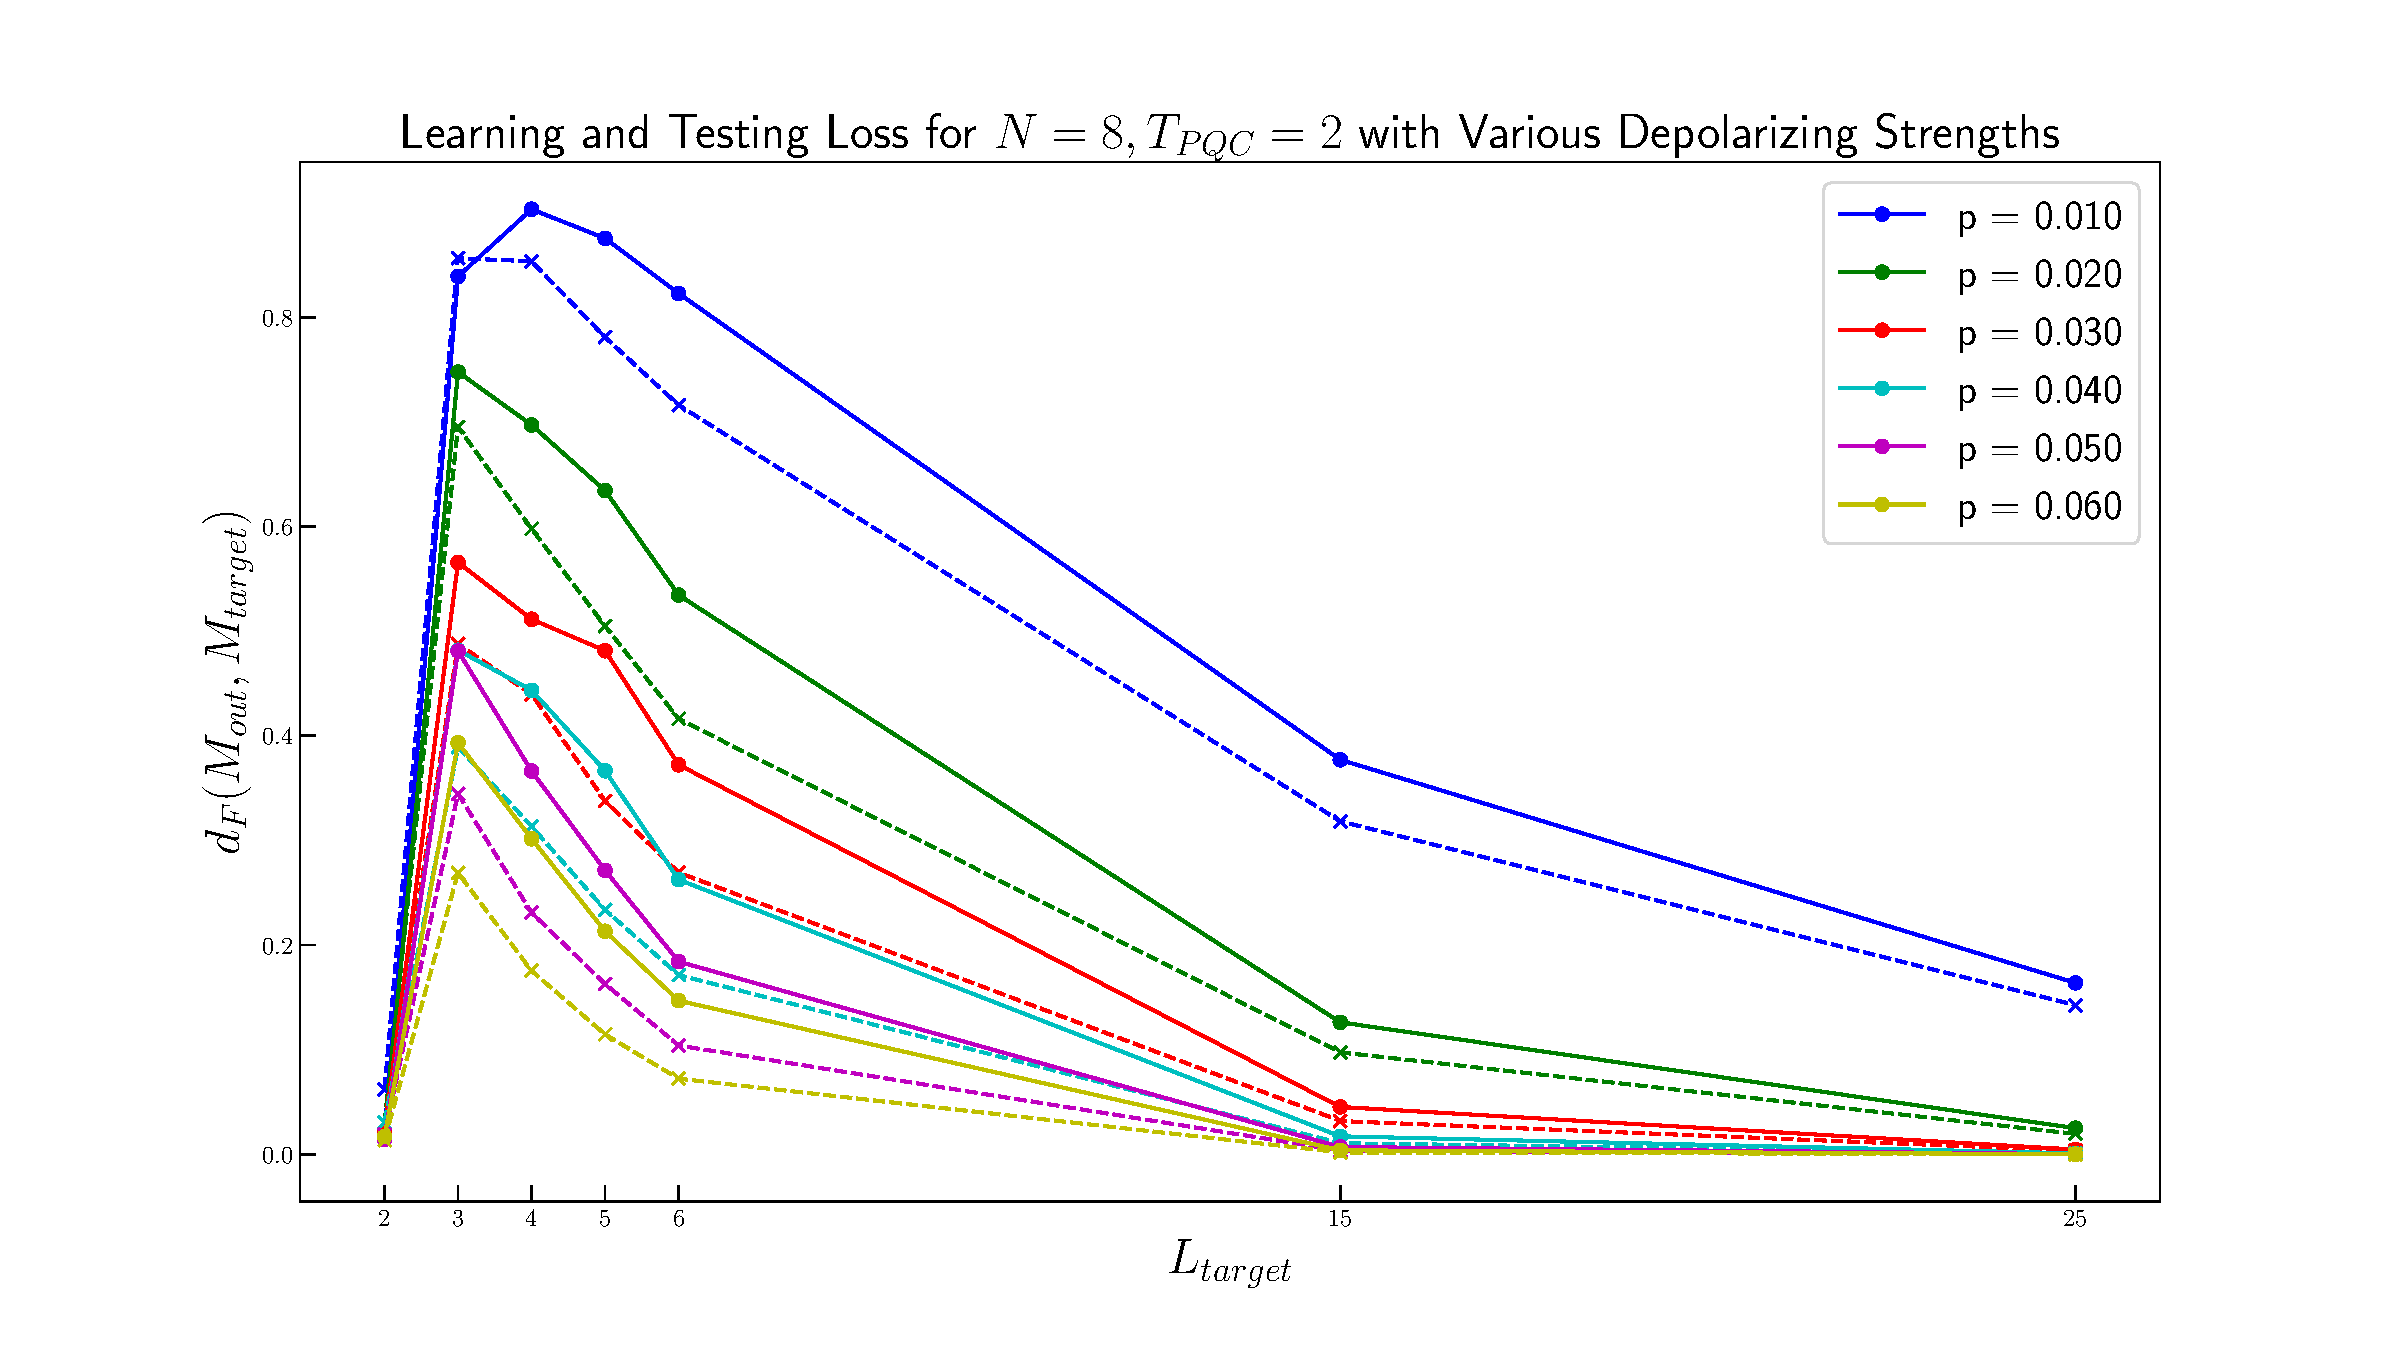
\includegraphics[width=\linewidth]{Depolarizing_ChangeT_N_L_p_8_2_all.pdf}
    \caption{}
    \label{fig:Depolarizing_ChangeT_N_L_p_8_2_all}
\end{subfigure}
\hfill
\begin{subfigure}{\linewidth}
    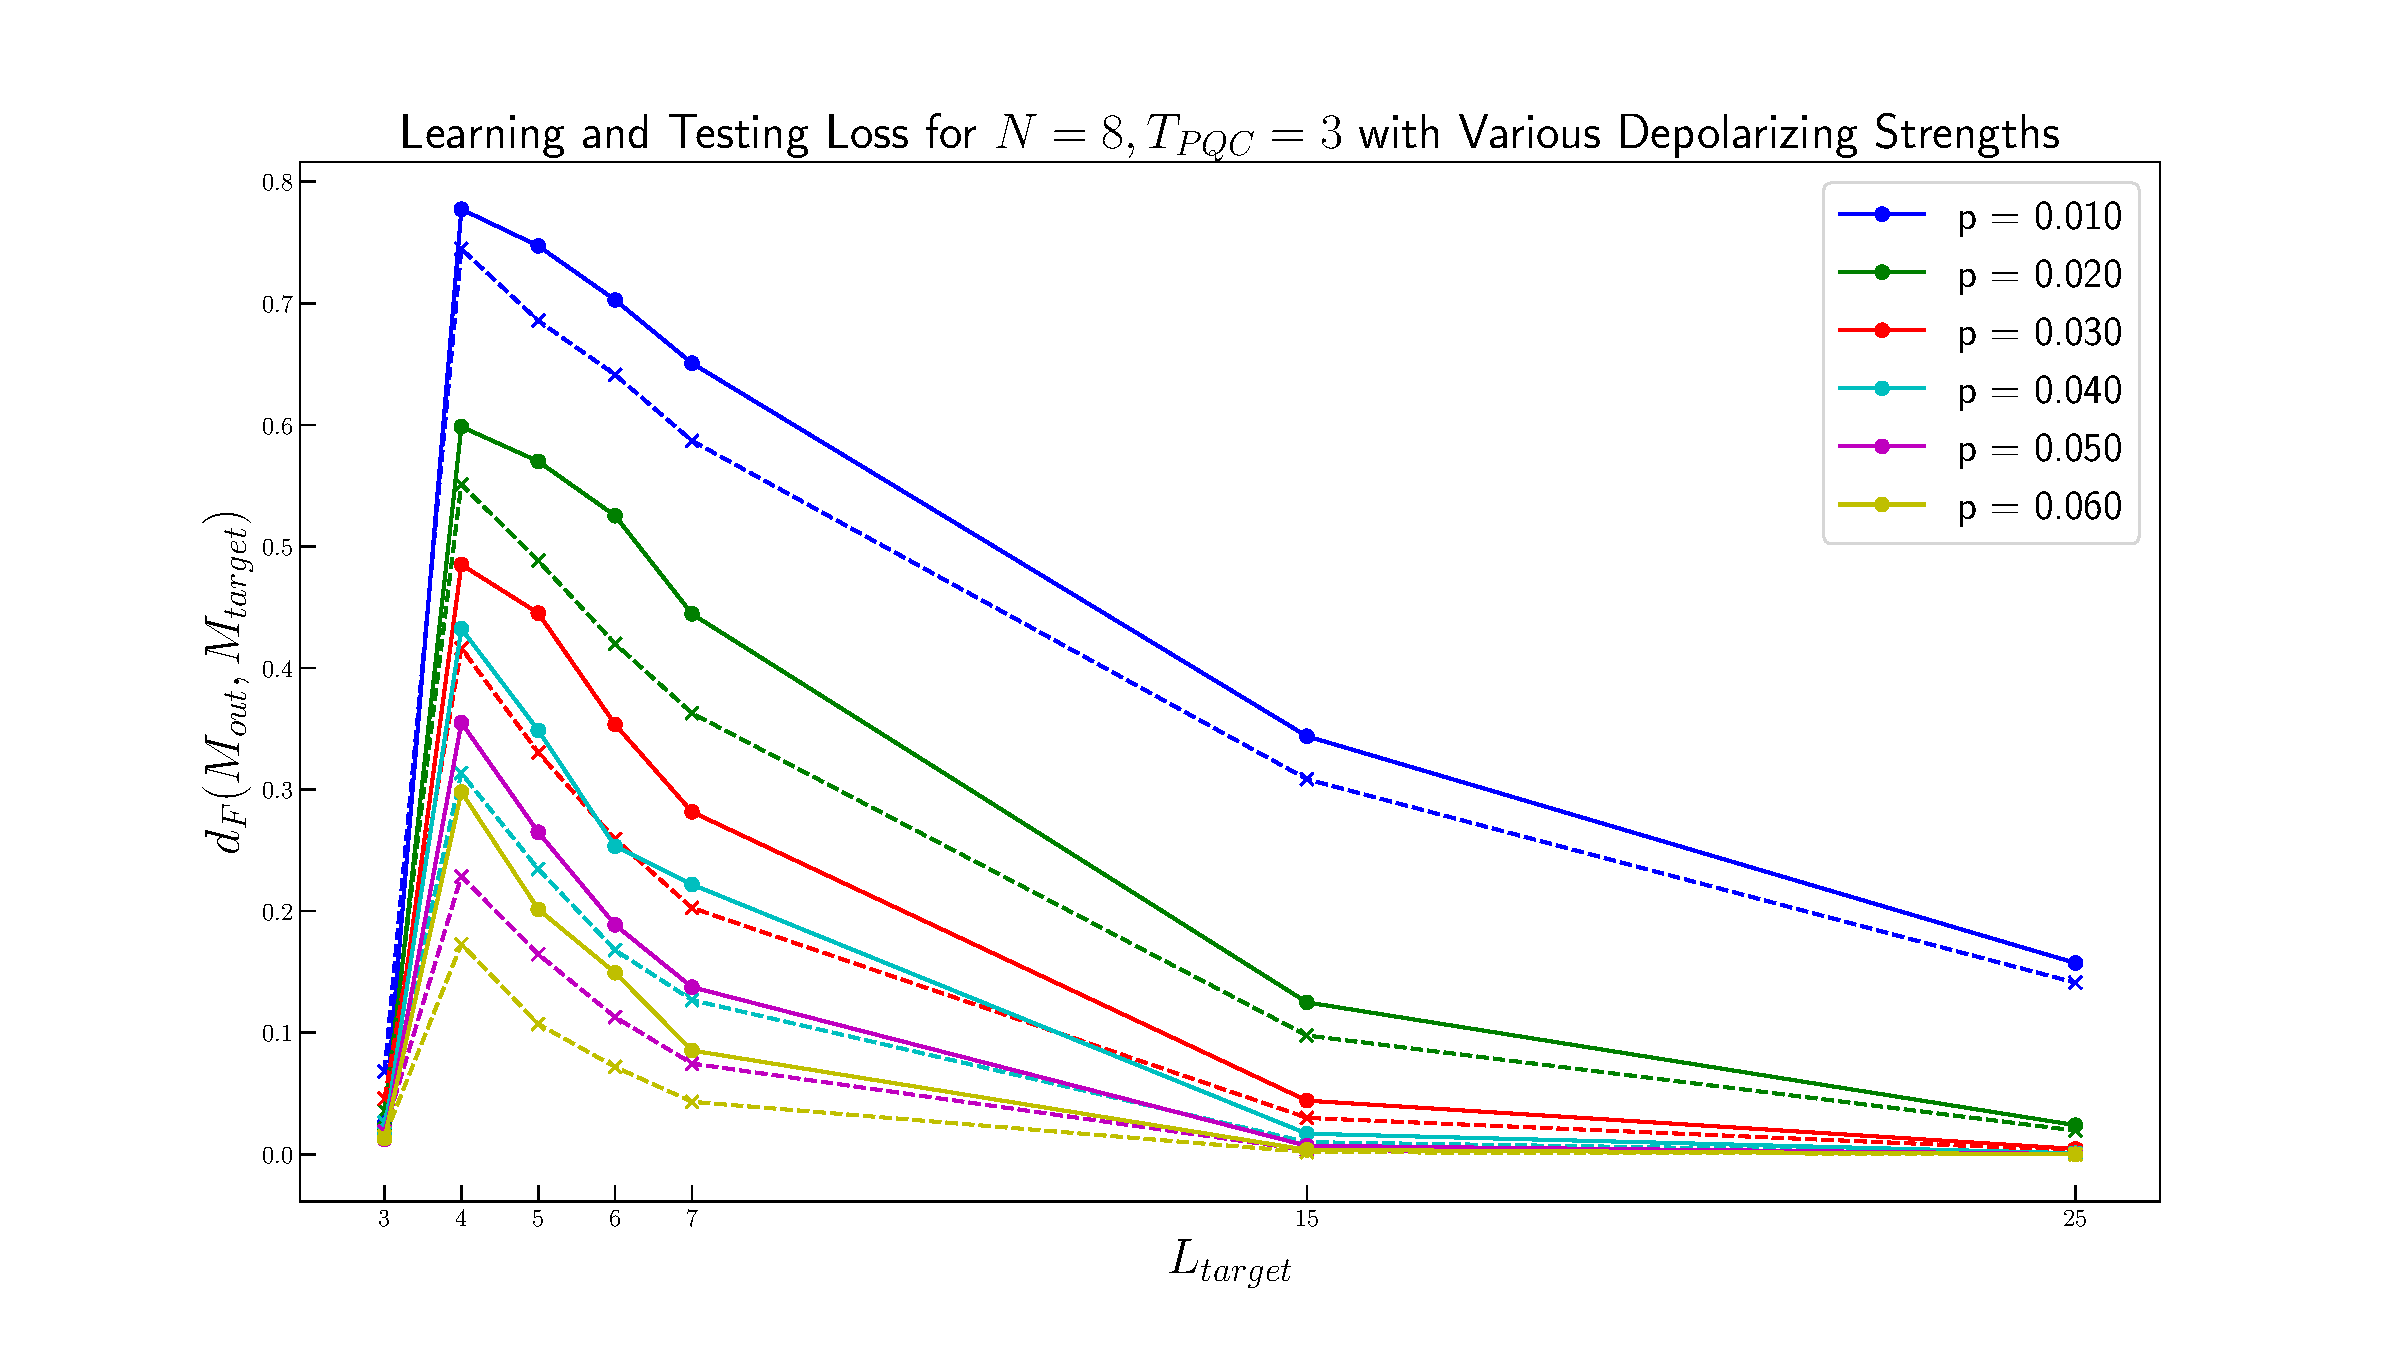
\includegraphics[width=\linewidth]{Depolarizing_ChangeT_N_L_p_8_3_all.pdf}
    \caption{}
    \label{fig:Depolarizing_ChangeT_N_L_p_8_3_all}
\end{subfigure}
\caption{\raggedright The learning result of using a shallower PQC with $N=8$ qubits to learn a random $L_{target}$-layer PQC with various depolarizing noise. Solid lines represent the final average learning loss with all weight-1 Pauli strings, and dashed lines represent the final testing loss for 200 randomly sampled Pauli strings. Sub-figure \textbf{(a)} uses a 2-layer PQC, and Sub-figure \textbf{(b)} uses a 3-layer PQC.}
\label{fig:Depolarizing_ChangeT_8}
\end{figure}

\begin{figure}
\centering
\begin{subfigure}{\linewidth}
    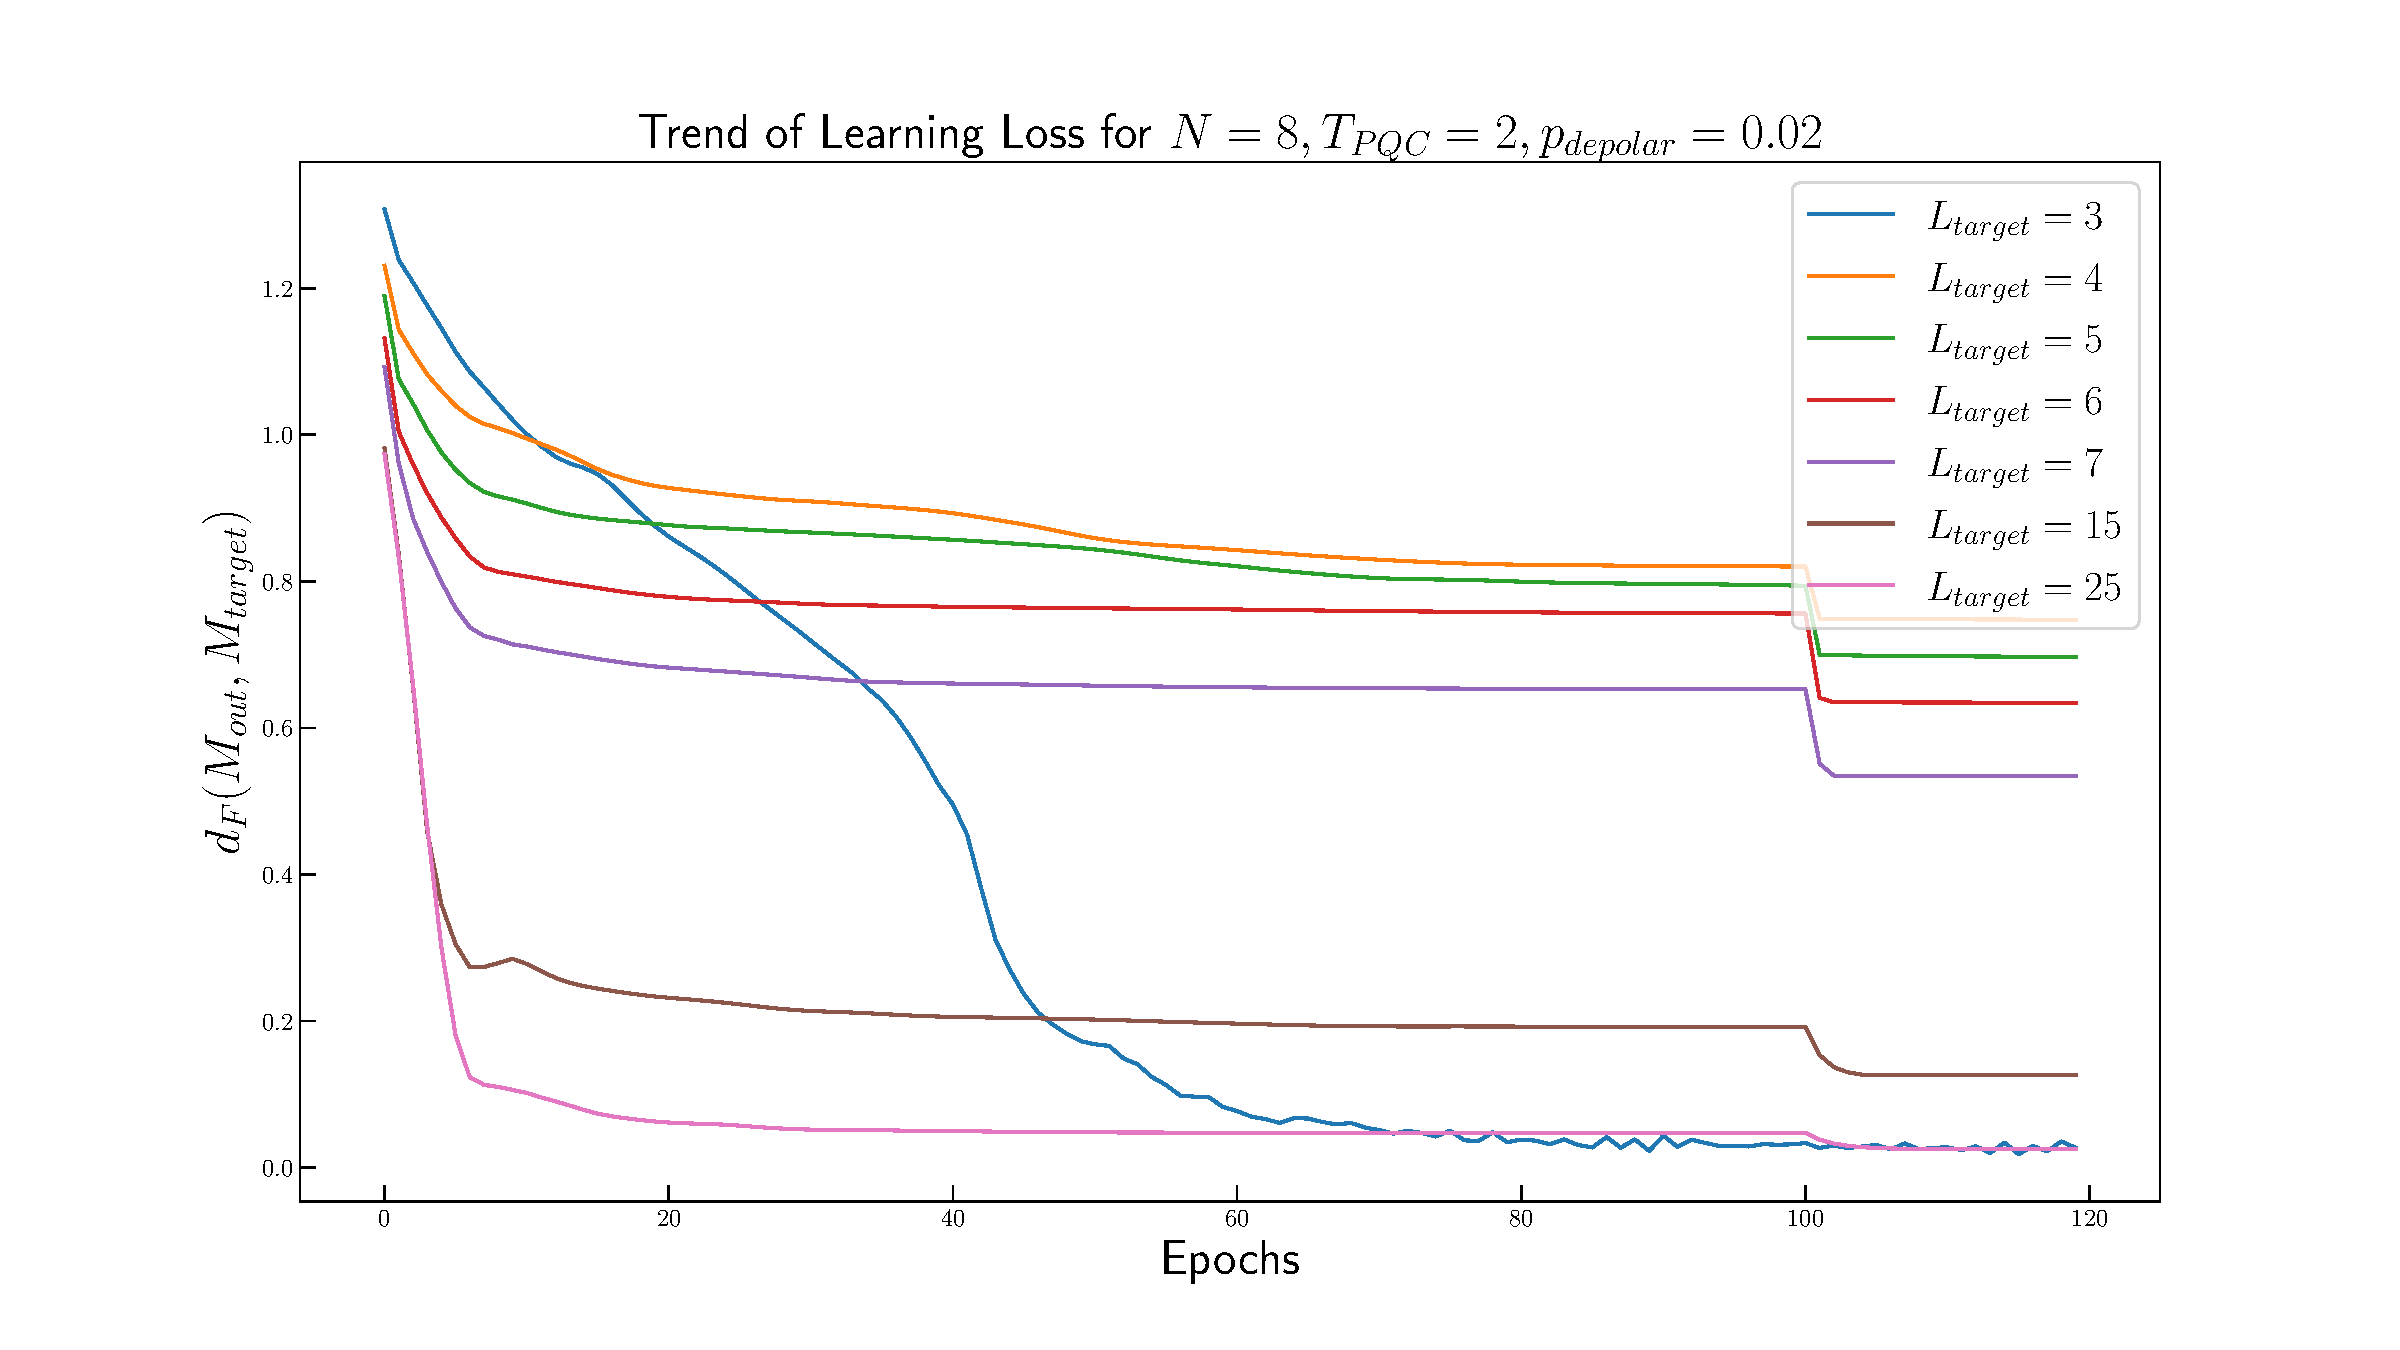
\includegraphics[width=\linewidth]{Depolarizing_learning_loss_trend_8_2_002.pdf}
    \caption{}
    \label{fig:Depolarizing_learning_loss_trend_8_2_002}
\end{subfigure}
\hfill
\begin{subfigure}{\linewidth}
    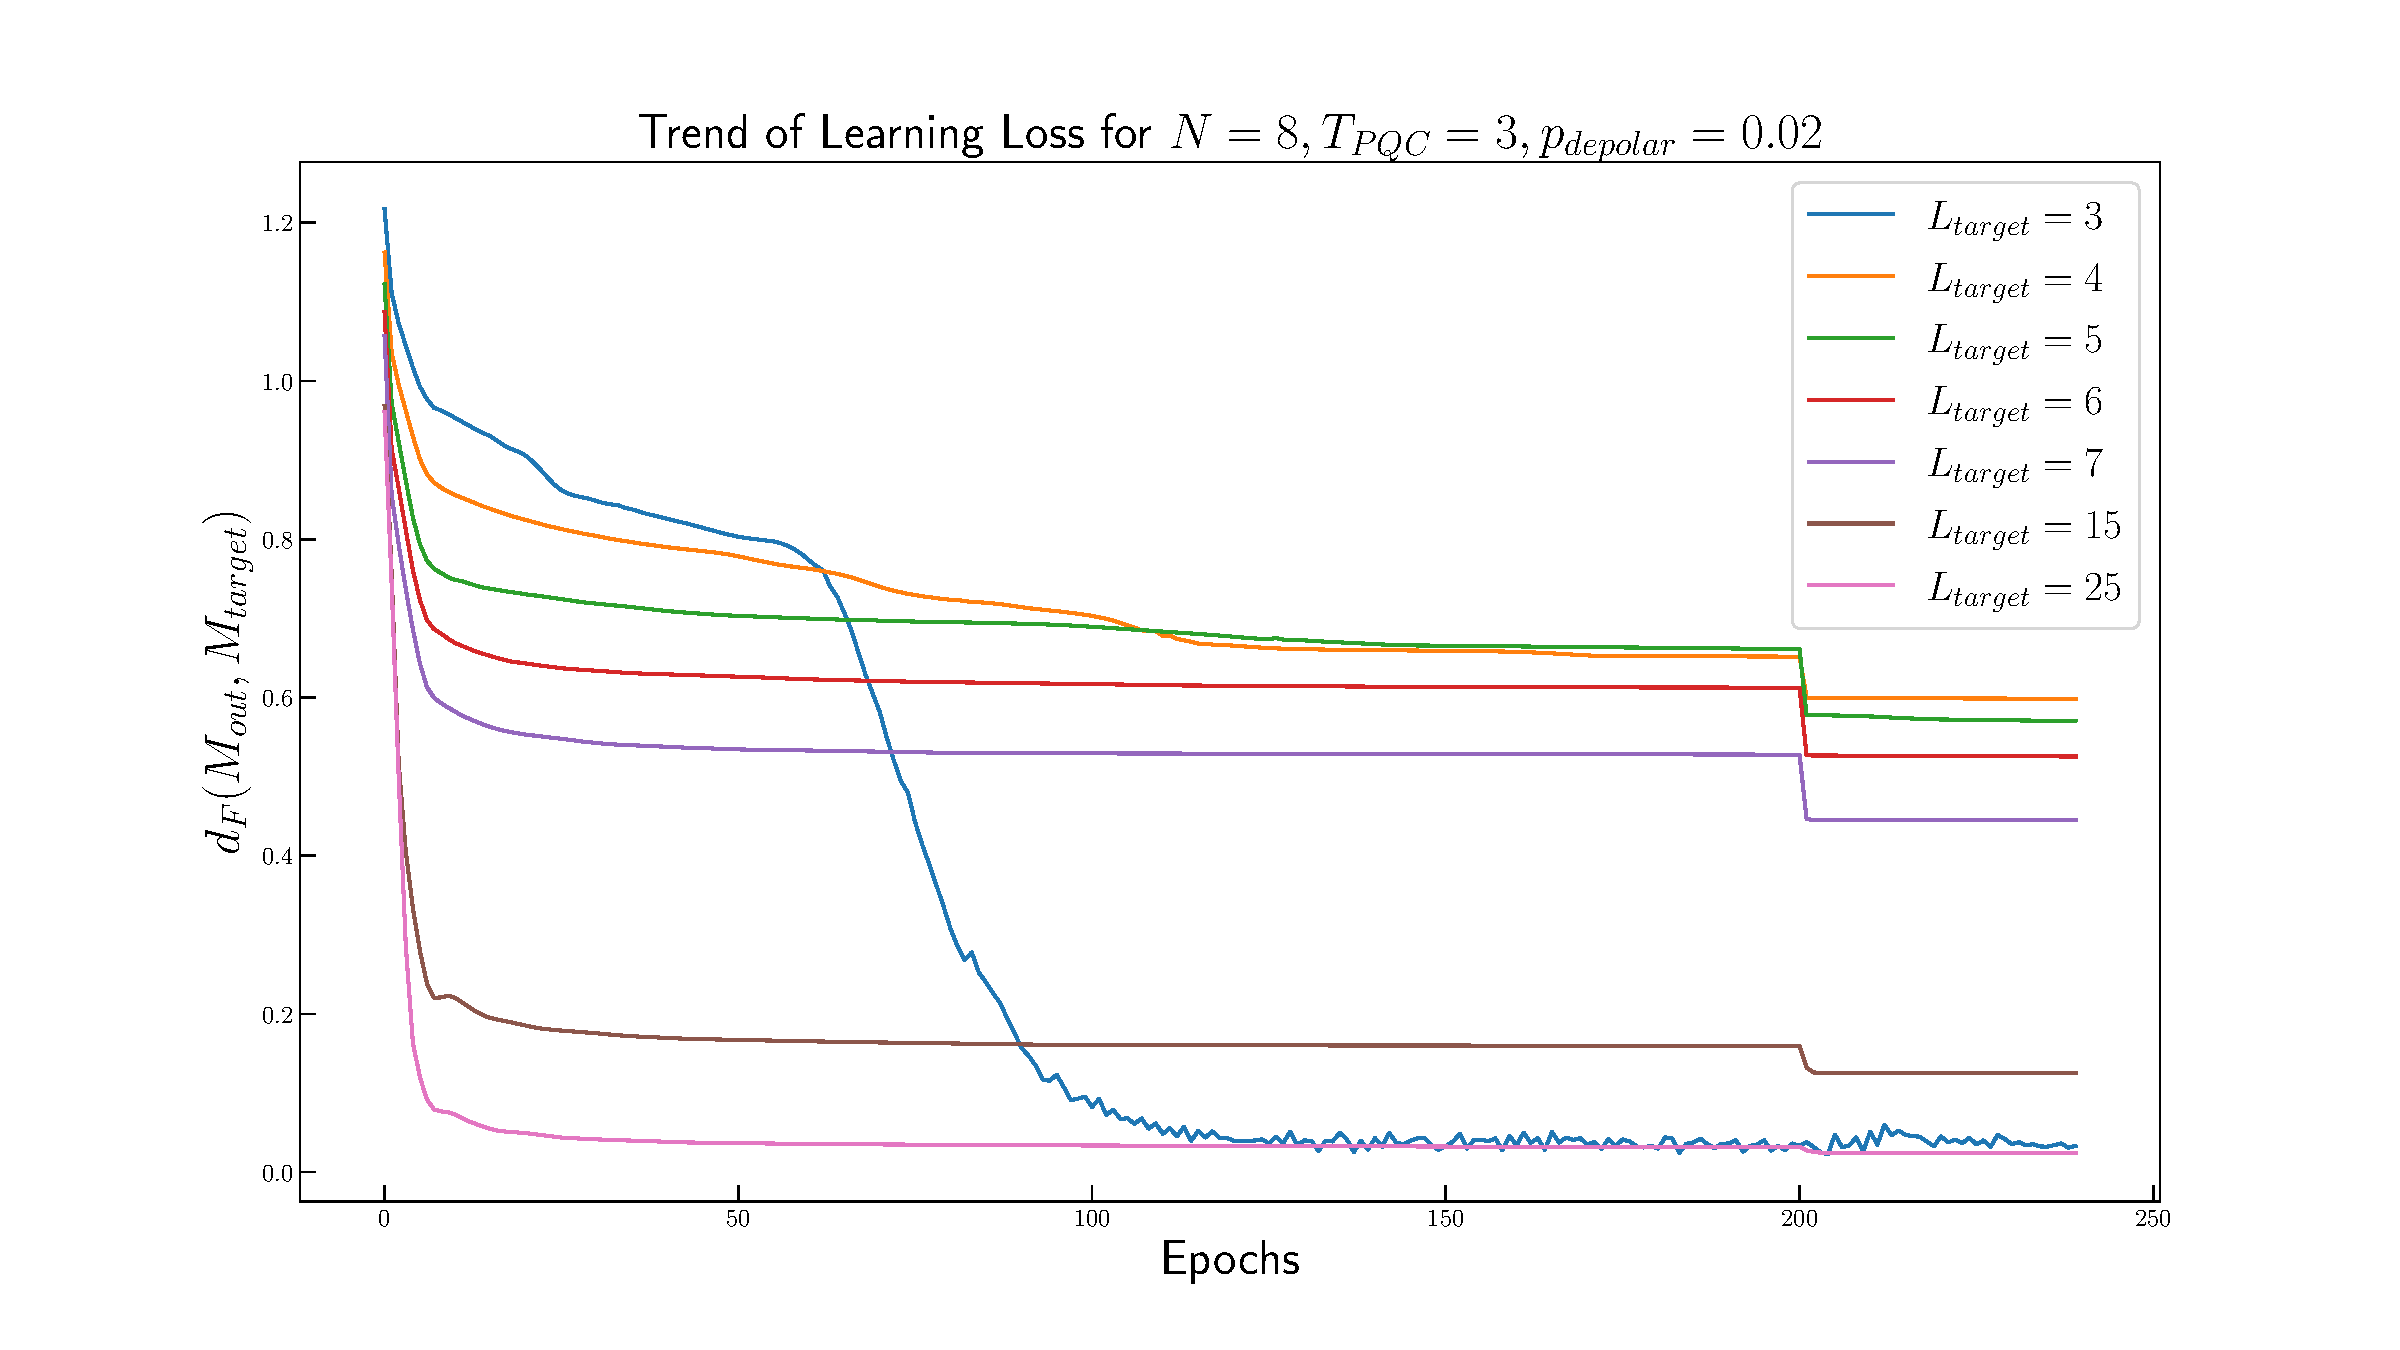
\includegraphics[width=\linewidth]{Depolarizing_learning_loss_trend_8_3_002.pdf}
    \caption{}
    \label{fig:Depolarizing_learning_loss_trend_8_3_002}
\end{subfigure}
\caption{\raggedright Example of the trend of the learning loss of using a shallower PQC to learn a random $L_{target}$-layer PQC with depolarizing probability $p_{depolar}=0.02$. Sub-figure \textbf{(a)} uses a 2-layer PQC and Sub-figure \textbf{(b)} uses a 3-layer PQC.}
\label{fig:Depolarizing_learning_loss_trend}
\end{figure}

Firstly, with the computational resources presented, the channel learning upto 8 qubits can be done without truncation. In Figure~\ref{fig:Depolarizing_ChangeT_8}, we demonstrated that using a 2-layer and a 3-layer PQC with moderate learning resources can effectively mimic a deeper circuit. The training is done with fewer than 200 epochs, and we notice that the convergence usually happens in the first 100 epochs. An example convergence training figure is shown in Figure~\ref{fig:Depolarizing_learning_loss_trend}. It is clear that when $T_{PQC}$ is smaller, it has faster convergence; however, all convergences are within a reasonable time, in about 200 epochs. 

The reason for the sudden drop in Figure~\ref{fig:Depolarizing_learning_loss_trend} at the final approximately $15\%$ of the training epochs is that, for the previous $85\%$, we restrict the maximum depolarizing noise in our model PQC to avoid the model getting stuck in a local minimum. If no restriction is imposed, the model PQC will quickly become a total depolarizing channel instead of learning the behaviours of the target channel.

\begin{figure}
\centering
\begin{subfigure}{\linewidth}
    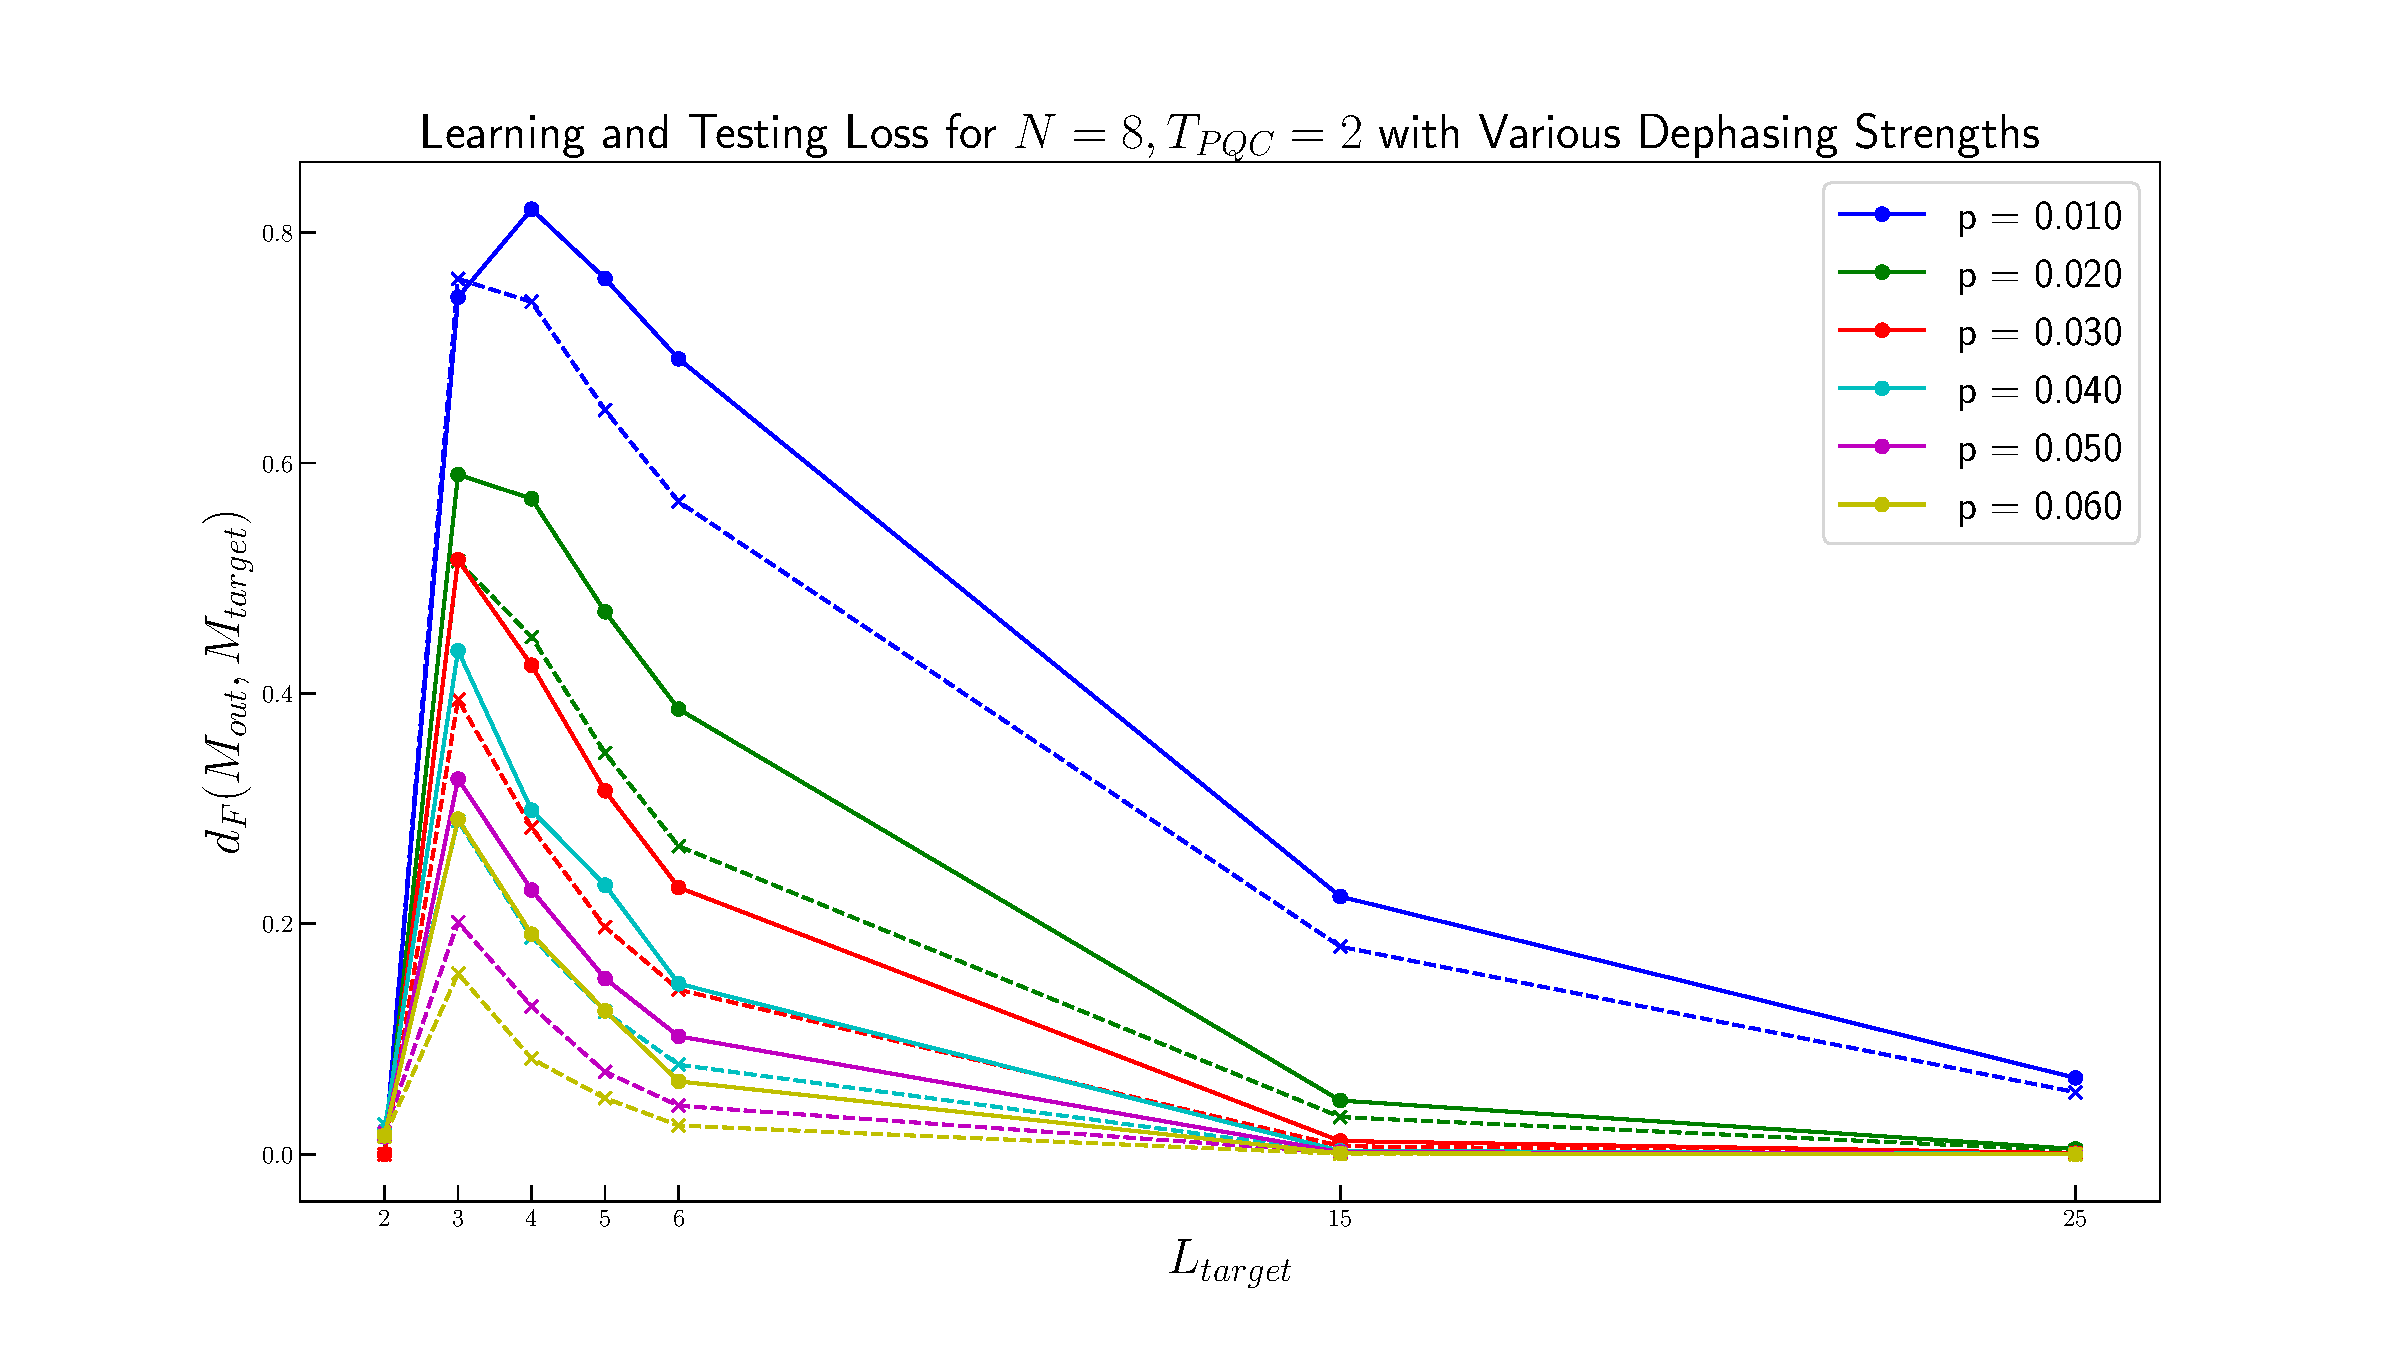
\includegraphics[width=\linewidth]{Dephasing_ChangeT_N_L_p_8_2_all.pdf}
    \caption{}
    \label{fig:Dephasing_ChangeT_N_L_p_8_2_all}
\end{subfigure}
\hfill
\begin{subfigure}{\linewidth}
    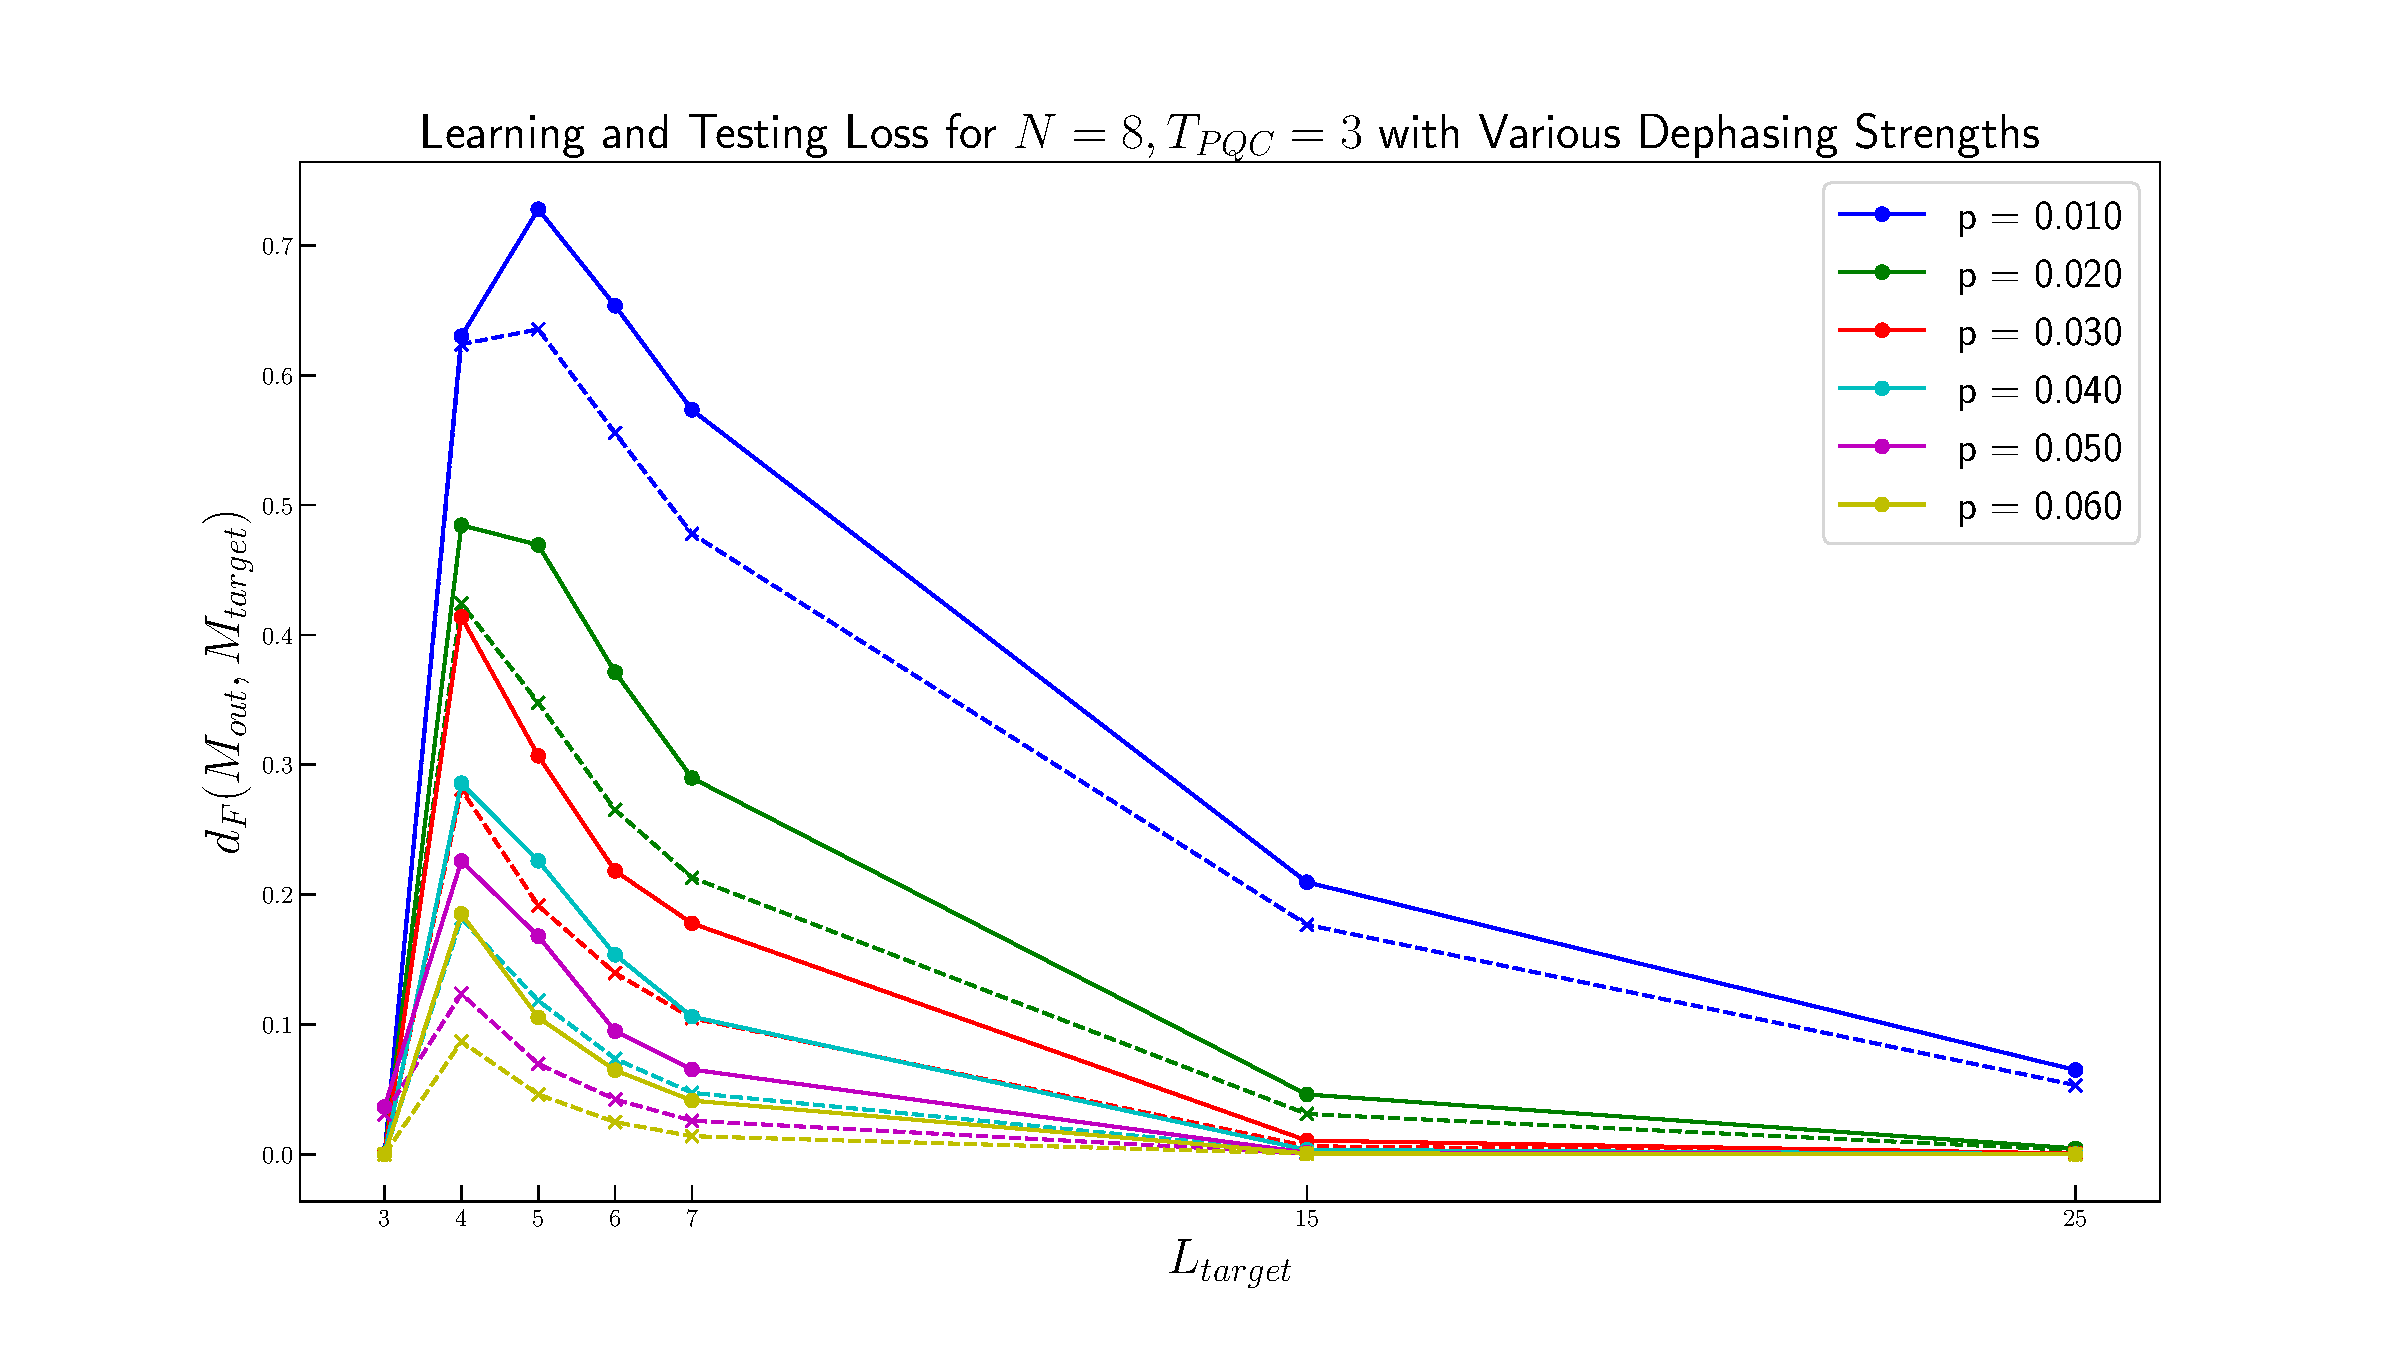
\includegraphics[width=\linewidth]{Dephasing_ChangeT_N_L_p_8_3_all.pdf}
    \caption{}
    \label{fig:Dephasing_ChangeT_N_L_p_8_3_all}
\end{subfigure}
\caption{\raggedright The learning result of using a shallower PQC with $N=8$ qubits to learn a random $L_{target}$-layer PQC with various dephasing noise. Solid lines represent the final average learning loss with all weight-1 Pauli strings, and dashed lines represent the final testing loss for 200 randomly sampled Pauli strings. Sub-figure \textbf{(a)} uses a 2-layer PQC, and Sub-figure \textbf{(b)} uses a 3-layer PQC.}
\label{fig:Dephasing_ChangeT_8}
\end{figure}

Similar learning results are obtained when we consider dephasing noise in the channel. Results are shown in Figure~\ref{fig:Dephasing_ChangeT_8}, where effective compression of a dephasing channel is possible, which significantly reduces the computational resources required for computation.

We emphasize that the above results are obtained without any truncation, ensuring their accuracy. 

\subsection{Results for 12 Qubits with Truncation}

\begin{figure}
\centering
\begin{subfigure}{\linewidth}
    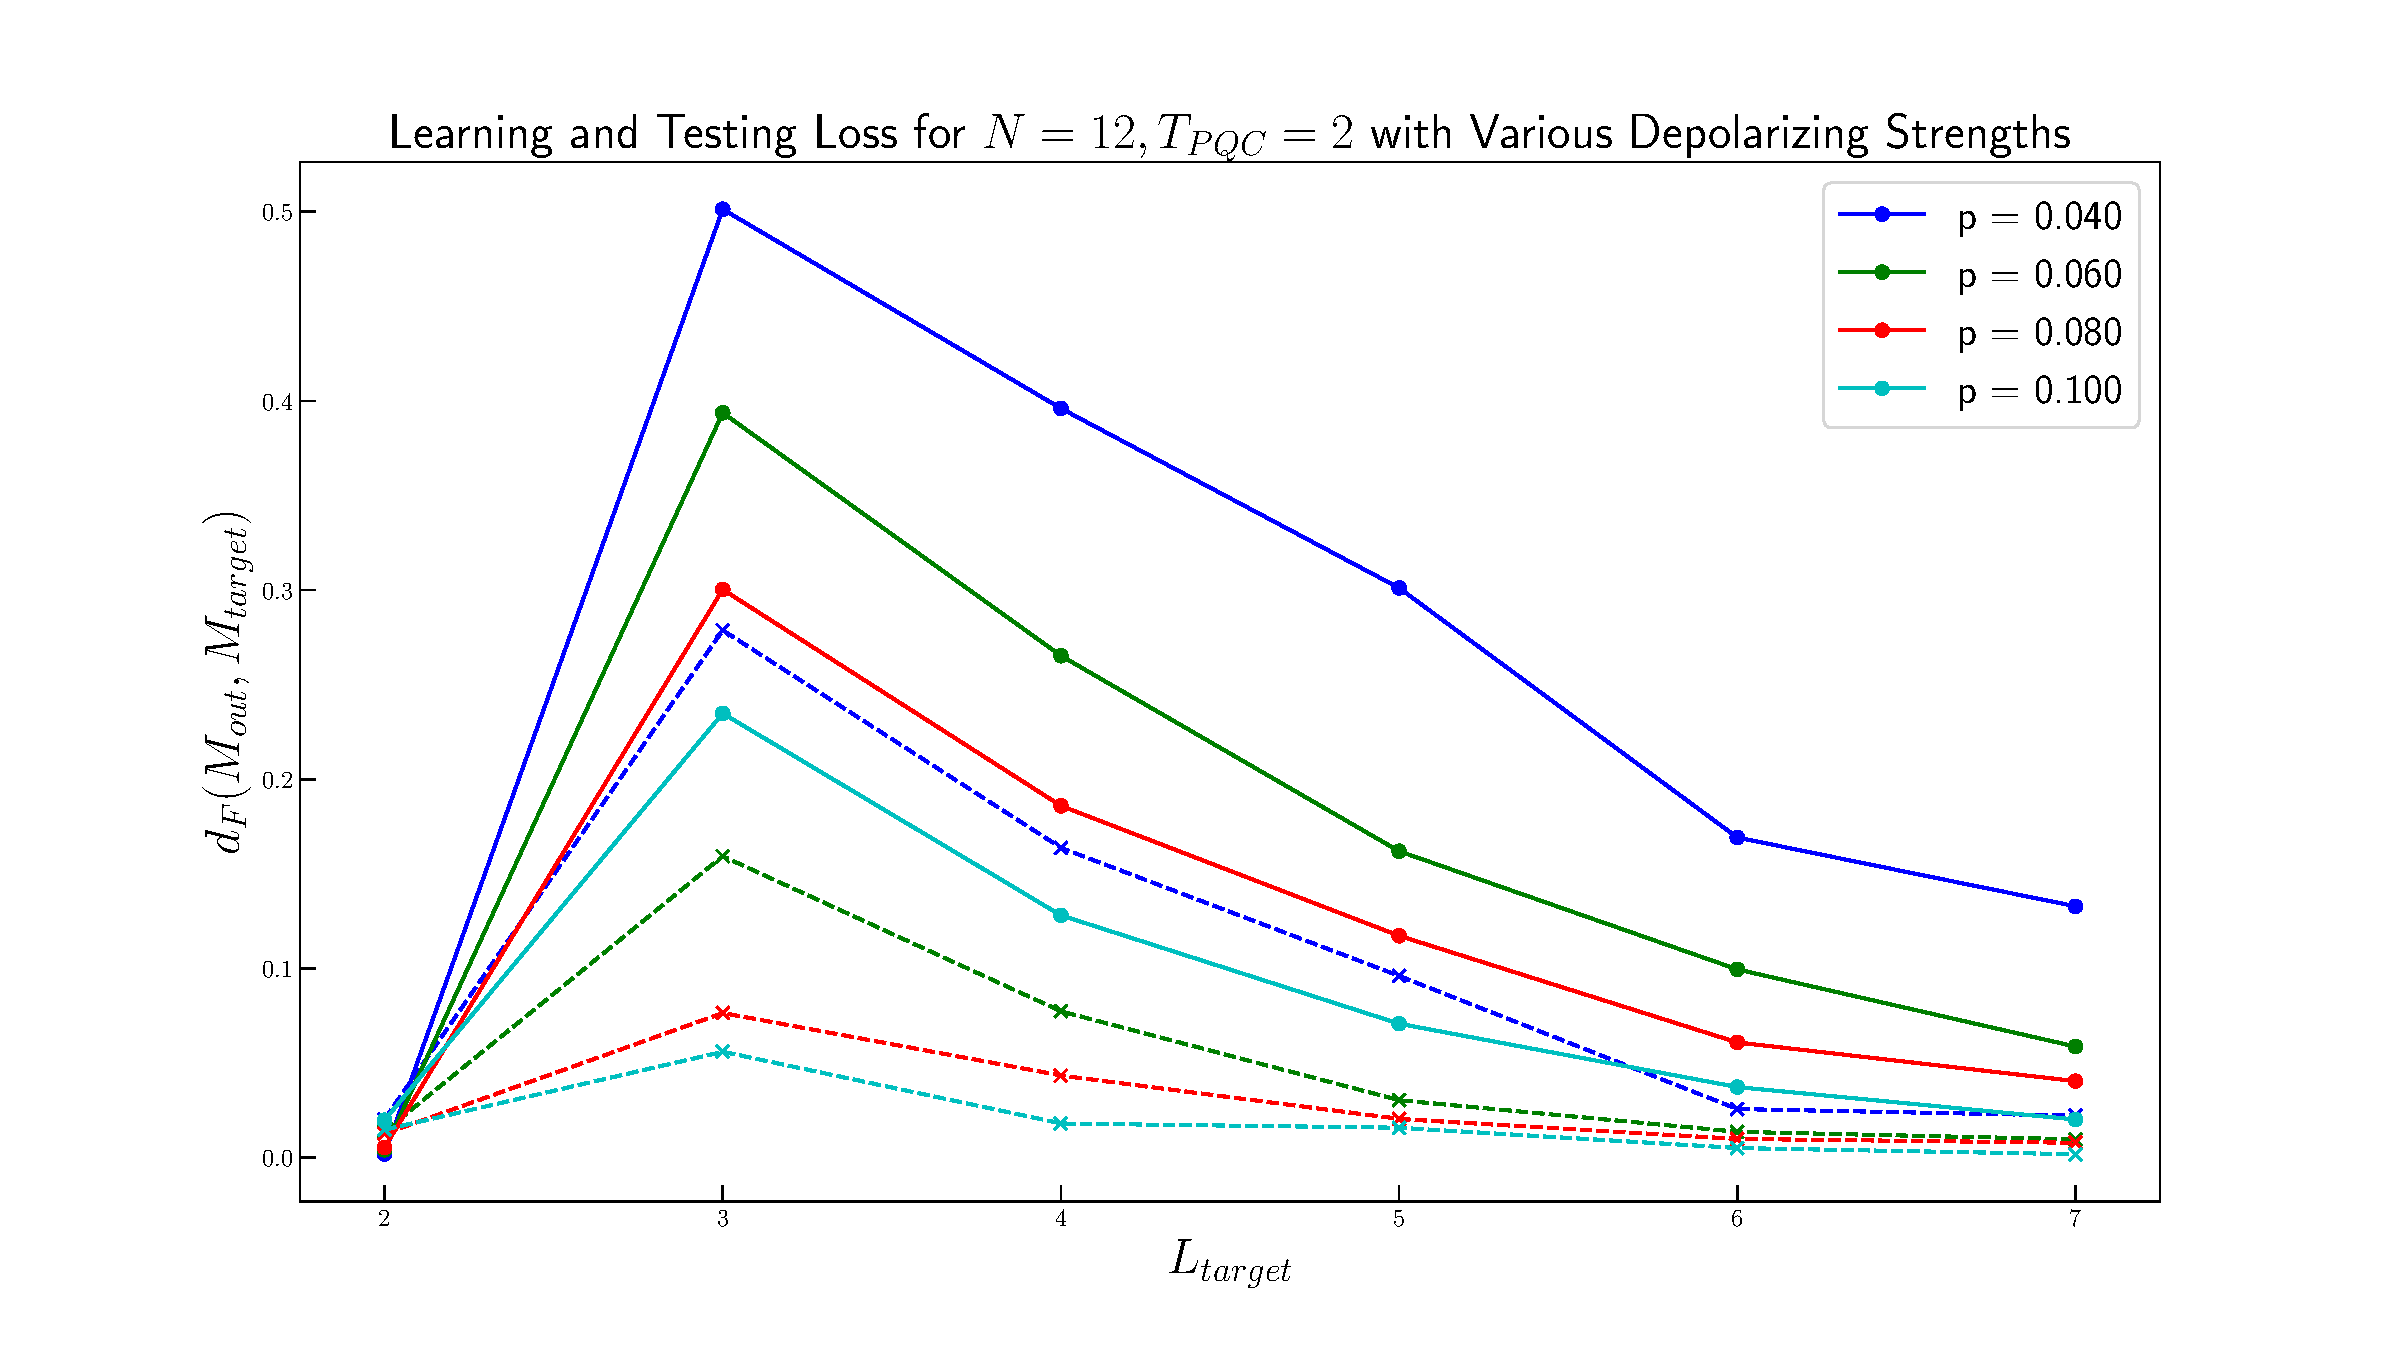
\includegraphics[width=\linewidth]{Depolarizing_ChangeT_N_L_p_12_2_all.pdf}
    \caption{}
    \label{fig:Depolarizing_ChangeT_N_L_p_12_2_all}
\end{subfigure}
\hfill
\begin{subfigure}{\linewidth}
    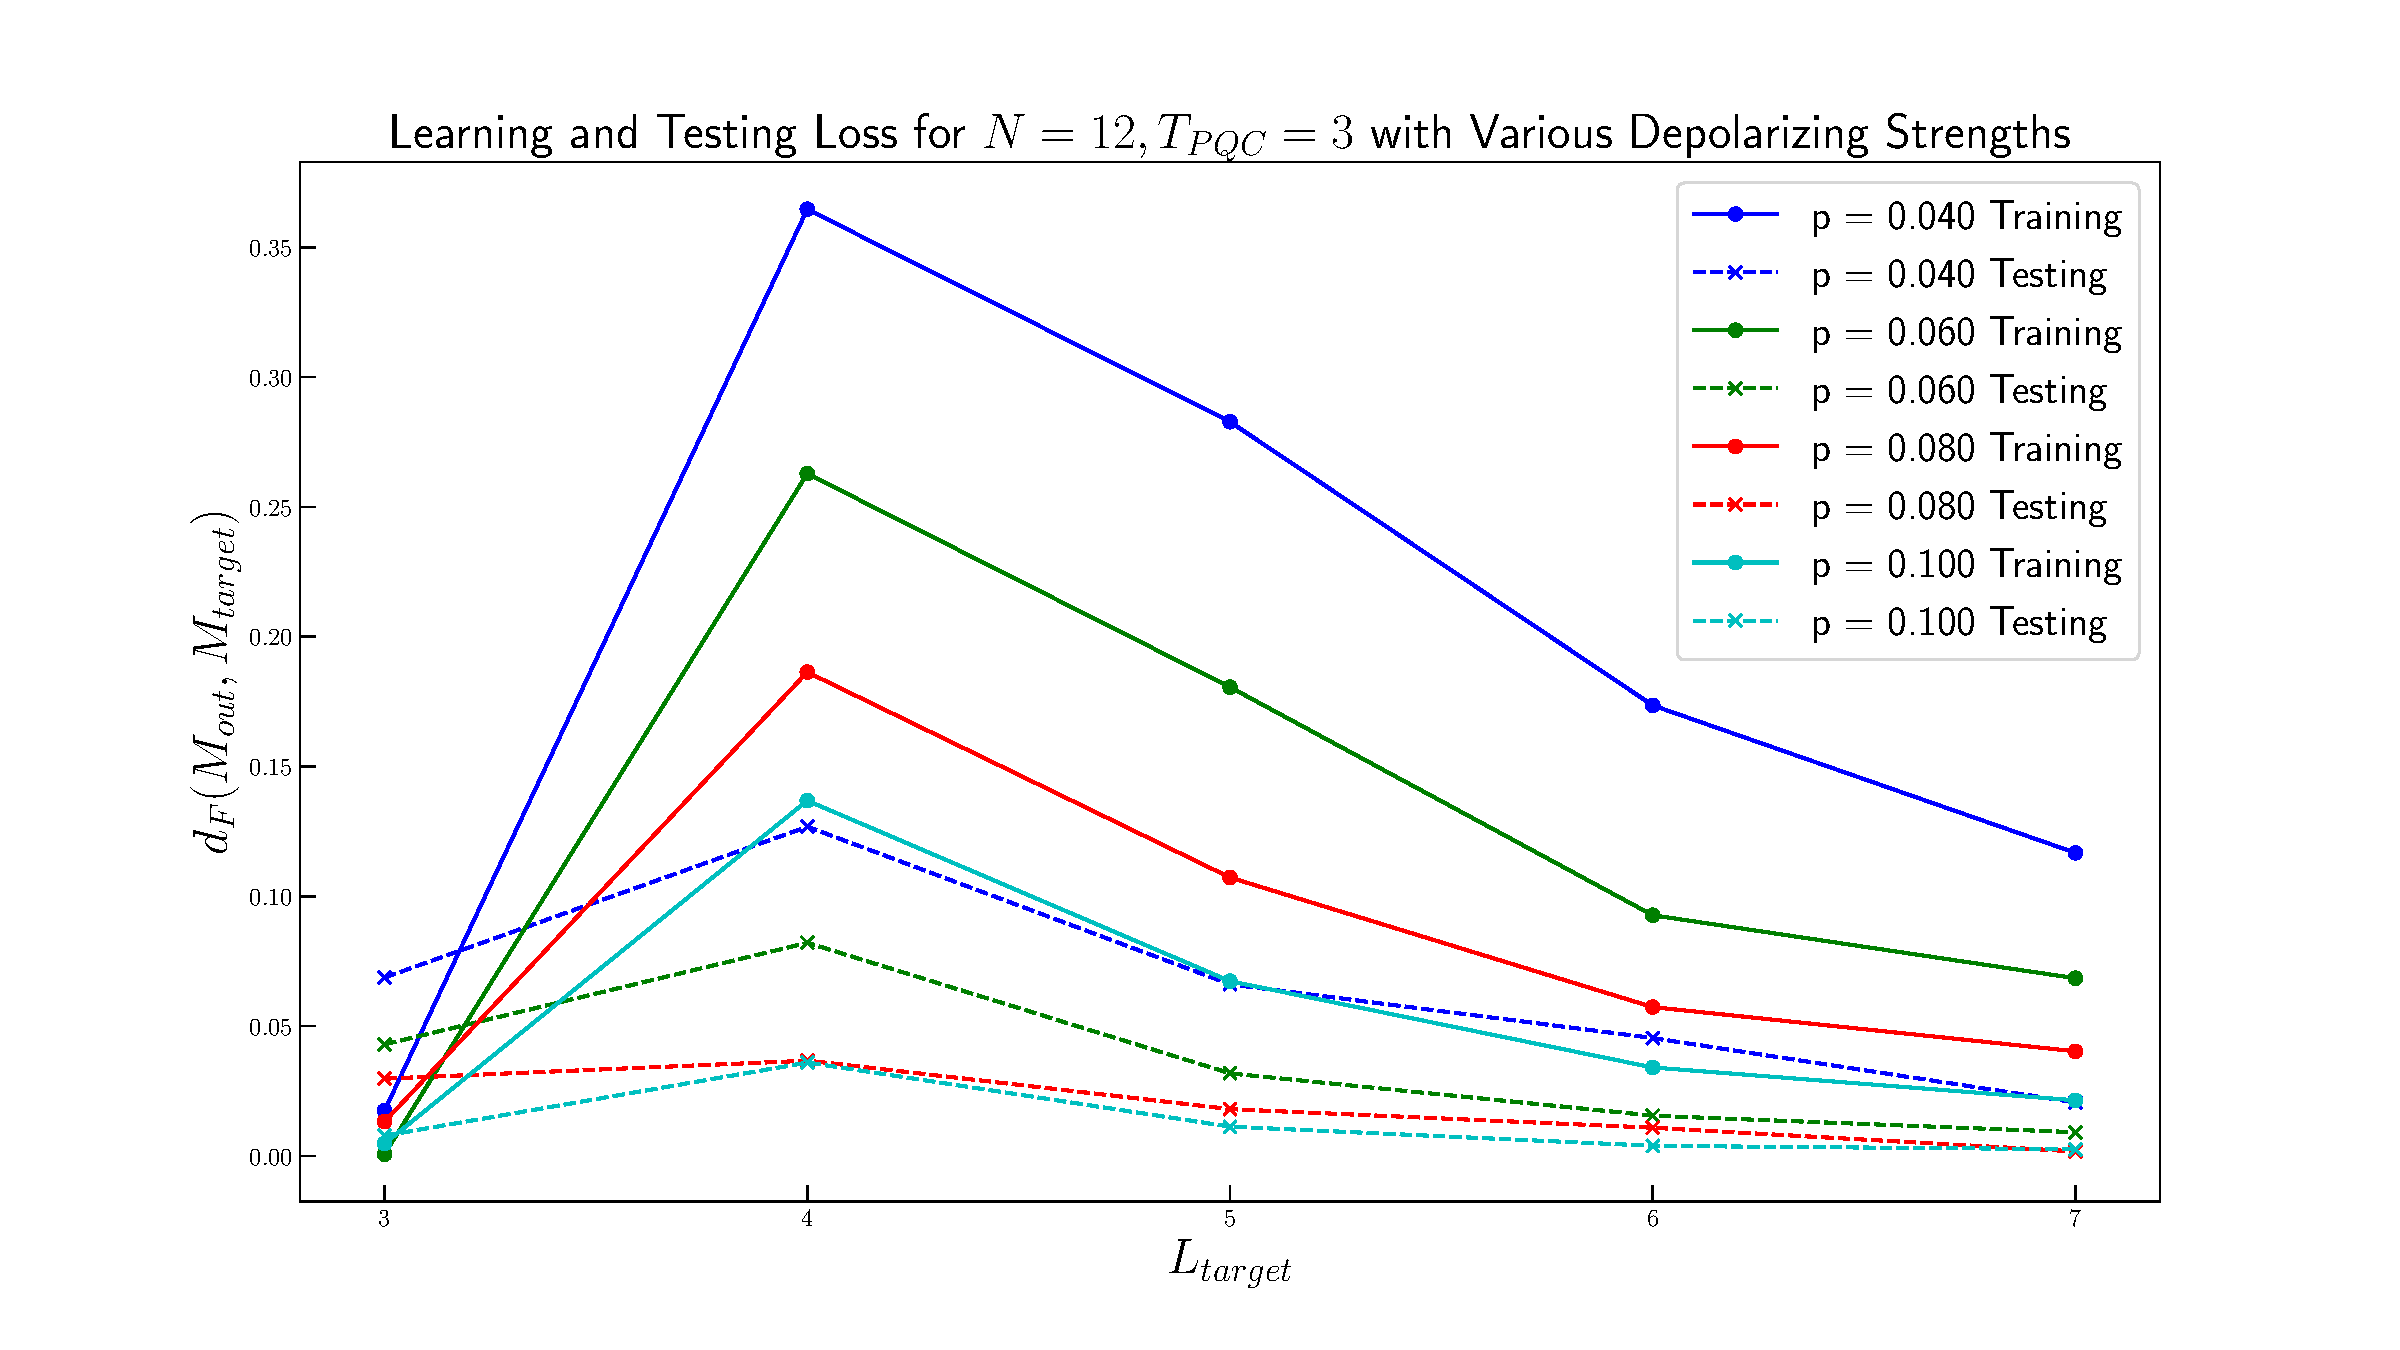
\includegraphics[width=\linewidth]{Depolarizing_ChangeT_N_L_p_12_3_all.pdf}
    \caption{}
    \label{fig:Depolarizing_ChangeT_N_L_p_12_3_all}
\end{subfigure}
\caption{\raggedright The learning result of using a shallower PQC with $N=12$ qubits with truncation $d_{max}=64, \epsilon_{cutoff}=10^{-5}$ to learn a random $L_{target}$-layer PQC with various depolarizing noise. Solid lines represent the final average learning loss with all weight-1 Pauli strings, and dashed lines represent the final testing loss for 200 randomly sampled Pauli strings. Sub-figure \textbf{(a)} uses a 2-layer PQC, and Sub-figure \textbf{(b)} uses a 3-layer PQC.}
\label{fig:Depolarizing_ChangeT_12}
\end{figure}

When propagating Pauli strings as an MPS through a general PQC, the bond dimension will grow exponentially with the depth and the number of qubits in the system. Therefore, truncation is needed for efficient learning. 

In our architecture, truncation is implemented by cutting the MPS bond dimensions after each layer of gates. We use the singular value decomposition (SVD) algorithm to perform the canonicalization of the MPS. When computing the SVD of each MPS site, we set a threshold on the maximum bond dimension $d_{max}$ kept and a cutoff singular value $\epsilon_{cutoff}$. For a bond between 2 MPS sites, all singular values below the cutoff $\epsilon_{cutoff}$ will be discarded. Then, if the bond dimension is still greater than the maximum bond dimension $d_{max}$, only the largest $d_{max}$ singular values at each bond will be kept.

However, when performing PQC learning without non-unitary noise, truncation will usually lead to significant truncation error. However, with small non-unitary noise, the small singular values at each MPS bond are significantly suppressed, and the truncation error becomes tolerable. 

In this subsection, we truncate the bond dimension of the MPS to $d_{max}=64$ and set $\epsilon_{cutoff}=10^{-5}$. To avoid significant truncation error, we set the lowest depolarizing probability for learning to $p_{depolar}=0.04$ and obtain a similar result.

Figure~\ref{fig:Depolarizing_ChangeT_12} shows the learning result of using a shallower PQC with $N=12$ qubits with truncation $d_{max}=64, \epsilon_{cutoff}=10^{-5}$ to learn a random $L_{target}$-layer PQC with various depolarizing noise. The general trend is the same as in the case of $N=8$ qubits. Therefore, we believe the results are general and can be applied to a larger number of qubits.

\subsection{Quantum Channel Learning with small depolarizing noise}

We demonstrated that the learning can be efficiently done with a small error rate per layer, specifically, if we add a per-layer depolarizing noise $p$ of a few percent, the learning can be done efficiently. While in most of the previous plots, if we use a $T_{PQC}$-layer, $T_{PQC}=2, 3$, PQC to learn a Haar random $L_{target}$-layer PQC, then usually the learning and testing loss will peak at $L_{target}=T_{PQC}+1$. Because, for $L_{target}=T_{PQC}$, the complexity of the model and the target circuits are the same, which means the model PQC should be able to learn the target PQC perfectly, and for $L_{target}\ge T_{PQC}+2$, the depolarizing or dephasing noise will override, and the learning loss will be reduced.

\begin{figure}
\centering
\begin{subfigure}{\linewidth}
    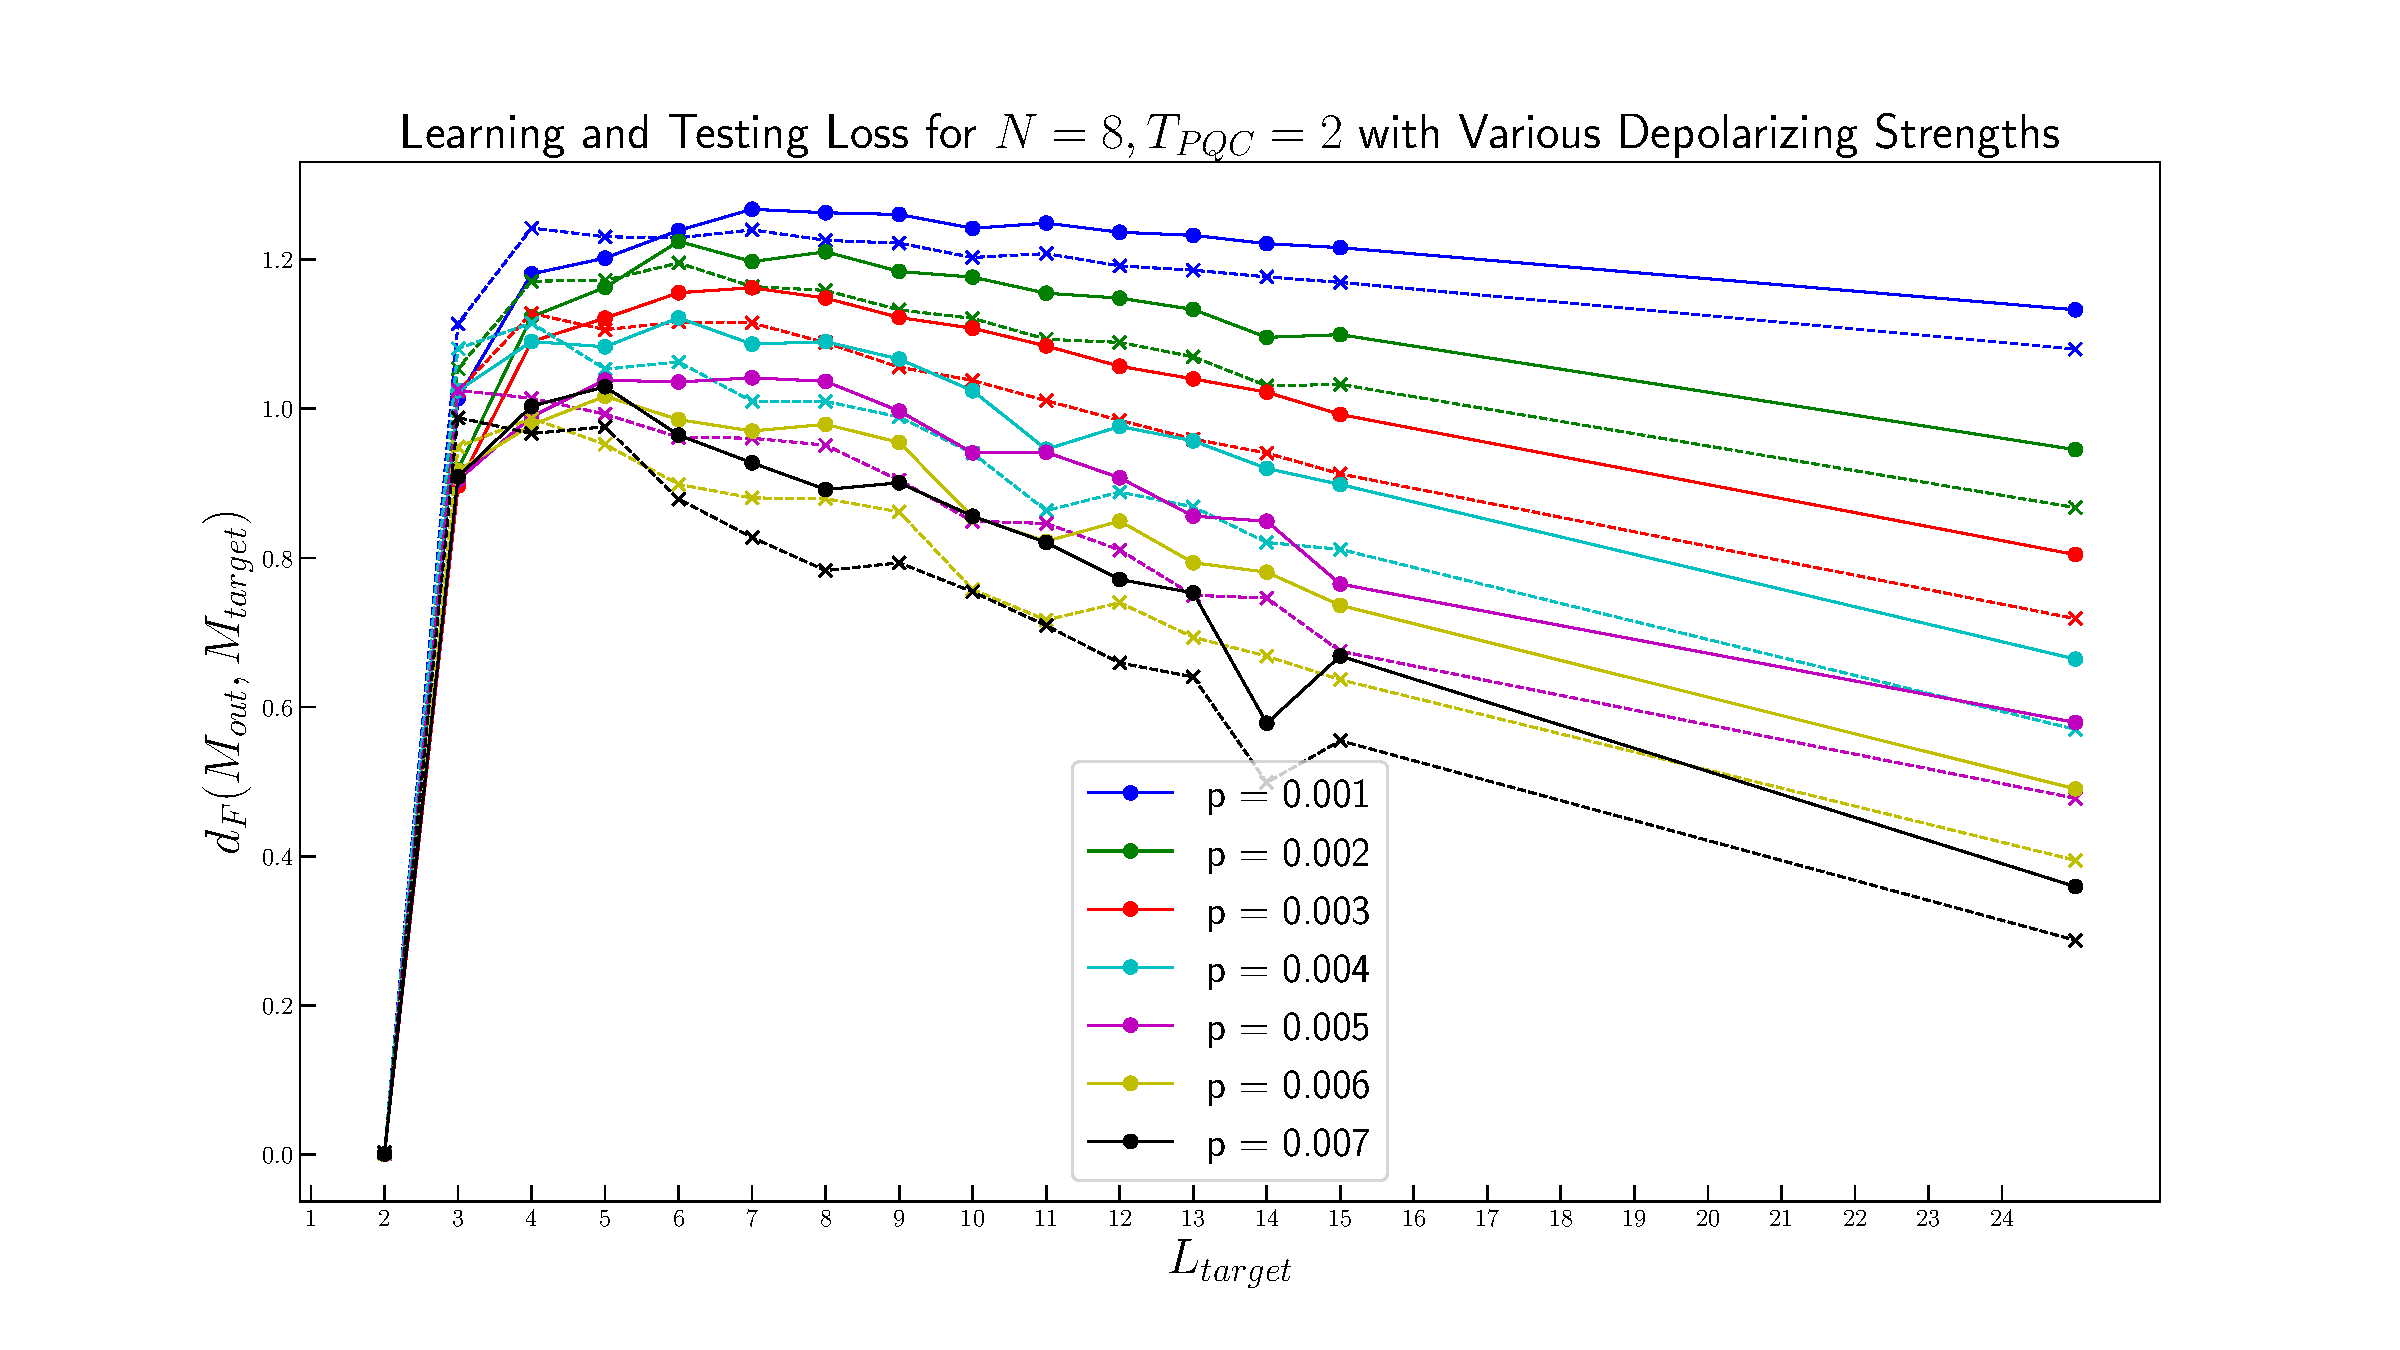
\includegraphics[width=\linewidth]{Dephasing_ChangeT_N_L_p_8_2_all_smallp.pdf}
    \caption{}
    \label{fig:Dephasing_ChangeT_N_L_p_8_2_all_smallp}
\end{subfigure}
\hfill
\begin{subfigure}{\linewidth}
    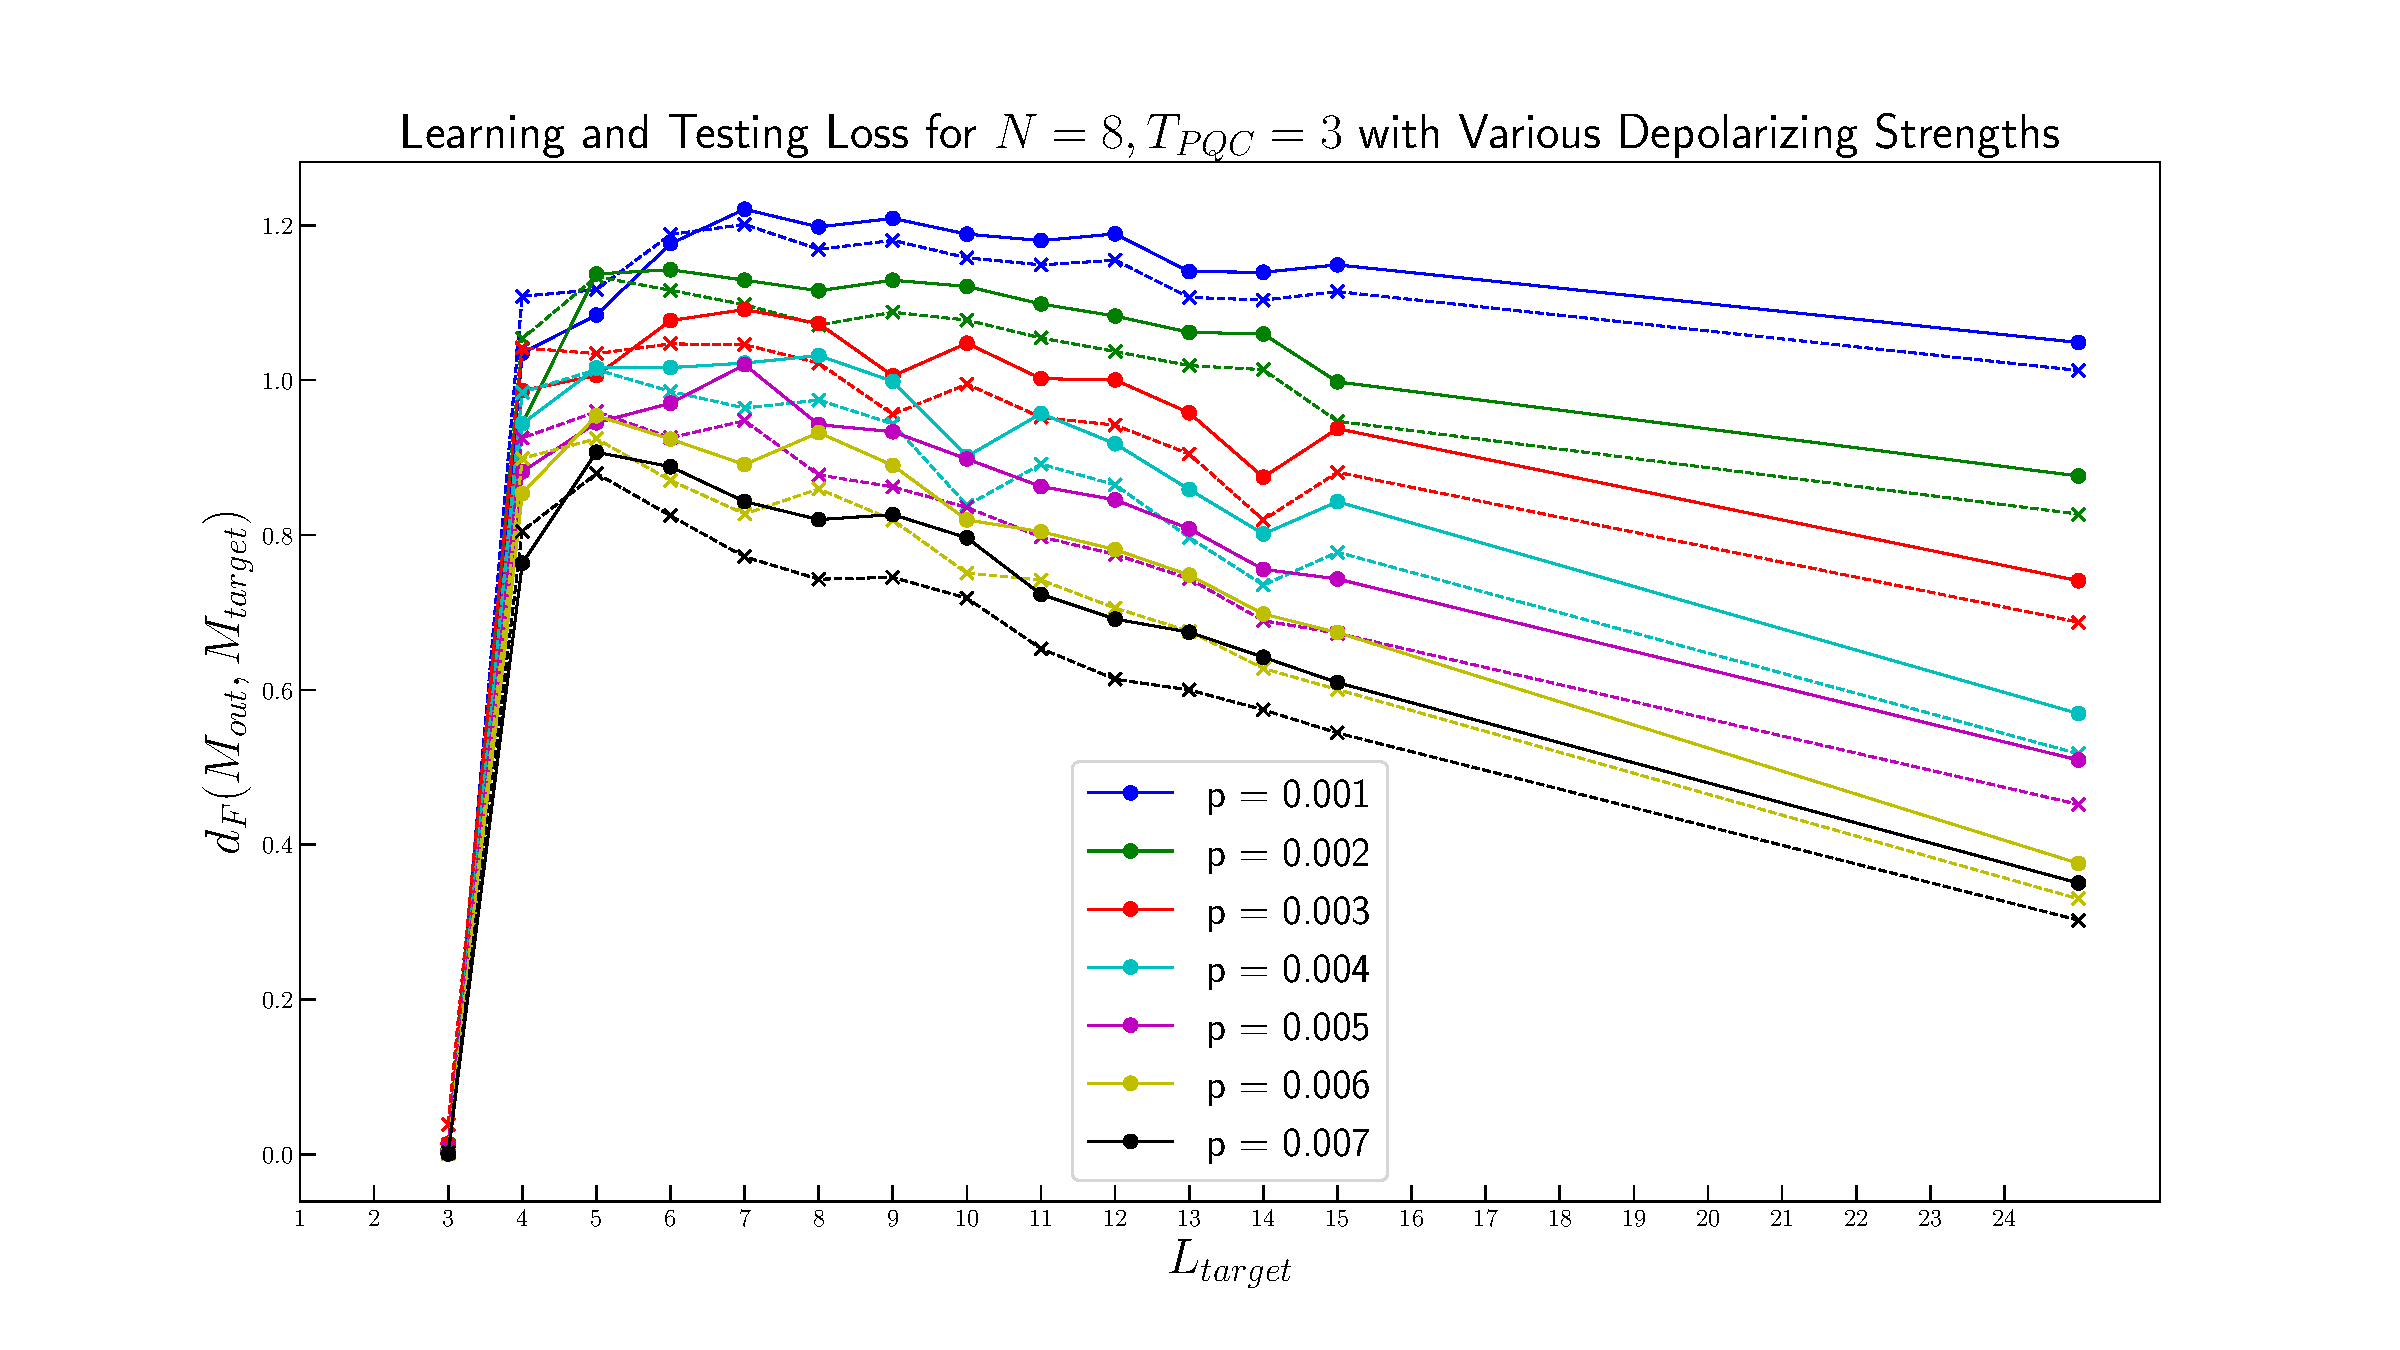
\includegraphics[width=\linewidth]{Dephasing_ChangeT_N_L_p_8_3_all_smallp.pdf}
    \caption{}
    \label{fig:Dephasing_ChangeT_N_L_p_8_3_all_smallp}
\end{subfigure}
\caption{\raggedright The learning result of using a shallower PQC with $N=8$ qubits to learn a random $L_{target}$-layer PQC with tiny depolarizing noise. Solid lines represent the final average learning loss with all weight-1 Pauli strings, and dashed lines represent the final testing loss for 200 randomly sampled Pauli strings. Sub-figure \textbf{(a)} uses a 2-layer PQC, and Sub-figure \textbf{(b)} uses a 3-layer PQC.}
\label{fig:Dephasing_ChangeT_8_smallp}
\end{figure}

However, this is not universal, since the complexity of PQC grows linearly with the number of layers until it saturates. At very small noise, we observe the shift in the peaked learning loss will shift from $L_{target}=T_{PQC}+1$ to $L_{target}=T_{PQC}+k$ for, roughly speaking, $k=2, 3, 4, 5$ depending on the noise level used, the explicit result is shown in Figure~\ref{fig:Dephasing_ChangeT_8_smallp}, where learning loss peaked at different $L_{target}$ for different depolarizing noise level used. Generally, the smaller the added depolarizing noise, the higher the shift of the peaked learning loss.

\section{Learning Lindbladian Dynamics}

In the previous section, we showed that random unitaries with noise can be compressed pretty well. And in this section, we shift our focus from random unitaries to some more useful physical systems. In which we consider the evolution of a generic one-dimensional quantum lattice with $n$ sites, labeled as $l\in\{1, \cdots, n\}$, each site situates a qubit in the two-dimensional Hilbert space $\mathbb{H}^2$, the same setup as the previous section, for arbitrary unitaries. Then, we model the evolution of the quantum lattice by a global density matrix $\rho$ with the Lindblad Master Equation.
\begin{equation}
\begin{split}
    \dot{\rho} &= \mathcal{L}[\rho]\\
    &=-\frac{i}{\hbar}[H, \rho]+\sum_{i}\gamma_i\left(L_i\rho L_i^\dagger - \frac{1}{2}L_iL_i^\dagger\rho- \frac{1}{2}\rho L_iL_i^\dagger\right)
\end{split}
\end{equation}

And, since our work focuses on learning the quantum channel in the operator basis, that is, in the Heisenberg picture. We present the Lindblad Master Equation in the Heisenberg picture with the operator $X$:

\begin{equation}
\begin{split}
    \dot{X} &= \mathcal{L}[X]\\
    &=\frac{i}{\hbar}[H, X]+\sum_{i}\gamma_i\left(L_iX L_i^\dagger - \frac{1}{2}L_iL_i^\dagger X- \frac{1}{2}X L_iL_i^\dagger\right)
\end{split}
\end{equation}

To retain the one-dimensional nature of the quantum lattice, we demand that the (time-dependent or independent) Lindbladian $\mathcal{L}$ only contains terms involving at most two nearest-neighbor interactions.
\begin{equation}
    \mathcal{L}[\rho]=\sum_l\mathcal{L}_{l, l+1}[\rho]
\end{equation}

The question we ask is whether useful Lindbladian dynamics can be efficiently learned and compressed in our setup, even in the presence of noise?

\subsection{Time-dependent master equation}

Following some classic examples, we consider a time-dependent master equation evolution of the states, which we start with a lattice of $n$ sites, and we load half of the sites with fermions and let the system evolve under a time-dependent Lindbladian:
\begin{equation}
    \mathcal{L}[X]=i[H, X]+\gamma \sum_{l=1}^n\left(n_l X n_l-\frac{1}{2} X n_l^2-\frac{1}{2} n_l^2 X\right)
\end{equation}
with the Hamiltonian defined as:
\begin{equation}
H = -J \sum_{l=1}^{n-1} \left( a_l^{\dagger} a_{l+1} + h.c. \right) - \mu(t) \left( \sum_{l=1}^{n/2} n_l - \sum_{l=n/2+1}^{n} n_l \right)
\end{equation}

To transform the Lindbladian into a quantum channel, we apply Trotterization of the Lindbladian dynamics into our simulation. 

\subsection{Thermal State Preparation}
One of the mixed states of wide interest in the community is the thermal state, which is specified by a nearest-neighbor Hamiltonian $H$ and an inverse temperature $\beta=1/k_BT$.
\begin{equation}
    \rho_\beta=\frac{e^{-\beta H}}{Z(\beta)}=\frac{1}{Z(\beta)}\sum_se^{-\beta E_s}\ket{E_s}\bra{E_s}
\end{equation}
Where the partition function $Z(\beta)=Tr(e^{-\beta H})$


\bibliography{Quantum_Channel_Learning}% Produces the bibliography via BibTeX.

\end{document}
%
% ****** End of file apssamp.tex ******
